% !TEX program = pdflatex --shell-escape

\documentclass[11pt]{article}
\usepackage[round,sort&compress,semicolon]{natbib}
\usepackage{times}
\usepackage[T1]{fontenc}
\usepackage[utf8]{inputenc}
\usepackage[pdftex]{graphicx}
\usepackage[letterpaper, left=1.0in, right=1.0in, top=1.0in, bottom=1.0in]{geometry}
\usepackage{ragged2e}
\usepackage{url}
\usepackage{setspace}
\usepackage{lineno}
\usepackage{multirow}
\usepackage{pdflscape}
\usepackage[backref=page]{hyperref}
\usepackage{hyperref}
\usepackage{rotating}
\usepackage{booktabs}
\usepackage[hypcap, labelsep=period, labelfont=bf]{caption}
\usepackage{array}
\usepackage{color}
\usepackage{soul}

\usepackage{amsmath}
\usepackage{amsfonts}       % blackboard math symbols
\usepackage{nicefrac}       % compact symbols for 1/2, etc.
\usepackage{microtype}      % microtypography
\usepackage{lipsum}		% Can be removed after putting your text content
\usepackage{doi}


\usepackage[usenames,dvipsnames,svgnames,table]{xcolor}
\hypersetup{
     colorlinks   = true,
     citecolor    = Indigo,
     linkcolor    = DarkCyan
}
\setlength{\RaggedRightParindent}{\parindent}
\linenumbers
\linespread{1.15}

%%% Add PDF metadata to help others organize their library
%%% Once the PDF is generated, you can check the metadata with
%%% $ pdfinfo template.pdf
\hypersetup{
	pdftitle={Waiting Distances Between Genealogy Changes under a Multi-Species Extension of the Sequentially Markovian Coalescent},
	pdfsubject={Evolutionary biology},
	pdfauthor={Patrick F. ~McKenzie},
	pdfkeywords={First keyword, Second keyword, More},
}

% \renewcommand{\shorttitle}{MSC Waiting Distance Distribution}

\begin{document}

\begin{center}
	{\bf \Large
		Estimating Waiting Distances Between Genealogy Changes under a \\[0.25cm]
		Multi-Species Extension of the Sequentially Markov Coalescent
	}\\[0.5cm]

	Patrick F. McKenzie$^{1}$ and Deren A. R. Eaton$^{1, *}$\\[0.25cm]

	\emph{
	$^{1}$ Department of Ecology, Evolution, and Environmental Biology, Columbia University, New York, NY 10027\\[0.5cm]
	$^{*}$ Contact: de2356@columbia.edu\\[0.5cm]
	}
\end{center}

% keywords can be removed
Keywords: Recombination, Phylogeny, SMC, Gene Tree, Species Tree, Concatalescence, ARG

\RaggedRight

\section*{Abstract}
Genomes are composed of a mosaic of segments inherited from different ancestors, 
each separated by past recombination events, and consequently, genealogical
relationships among multiple genomes vary spatially across different genomic 
regions. Expectations for the amount of genealogical variation among unlinked 
(uncorrelated) genomic regions is well described for either a single 
population (coalescent) or multiple structured populations (multispecies coalescent).
However, the expected similarity among genealogies at linked regions of a 
genome is less well characterized. 
Recently, an analytical solution was developed for the expected 
distribution of waiting distances between changes in genealogical trees 
spatially across a genome for a single population with constant effective 
population size. Here, we describe a generalization of this 
result, in terms of the expected distribution of waiting distances between 
changes in genealogical trees, and topologies, for multiple structured populations
with branch-specific effective population sizes (i.e., under the multispecies 
coalescent). Our solutions establish an expectation for genetic linkage  
in multispecies datasets, and provide a new likelihood framework for 
fitting species tree models \hl{to sequence data}.

\section{Introduction}

%It is well known that, because of recombination and random sorting at coalescence events, different locations in the genome might have different genealogical histories. In population genetics, the genealogical history of a set of samples at a neutrally evolving location in the genome can be modeled using the coalescent. In phylogenetics, genealogical histories are instead modeled with an extension of the coalescent known as the "multispecies coalescent." While the standard form of the coalescent assumes a single population with a constant effective population size, the multispecies coalescent incorporates species divergence time parameters to define a "species tree" topology, and each branch of the species tree has its own effective population size.

The multispecies coalescent (MSC) is an extension of the coalescent 
\citep{kingman1982coalescent}, a model that describes the distribution of genealogical 
histories among gene copies from a set of sampled individuals. Whereas the 
coalescent models a single panmictic population, the MSC includes constraints that prevent 
samples from different lineages from sharing a most recent genealogical ancestor until prior
to a species divergence event that separates them \citep{maddison1997gene,maddison2006inferring}. 
Conceptually, the MSC can be viewed as a piecewise model composed of the standard
coalescent applied to each interval of a "species tree", representing the relationships
and divergence times among isolated lineages. Genealogies are constrained to be
embedded within species trees (Fig.~\ref{fig:fig1}), and the joint likelihood of 
MSC model parameters can be estimated from the coalescent times among a 
distribution of sampled genealogies
% Analytically, the MSC can be viewed as a piecewise likelihood function composed of the 
% standard coalescent applied to each edge of a “species tree”, representing 
%a hierarchical model of 
% the relationships and divergence times among constraining lineages -- i.e., it can 
% be used to calculate the likelihood of a container tree within which a distribution of 
% genealogies must be embedded 
% Consider referencing a panel of a figure here to show genealogical embedding.
\citep{rannala2003bayes,degnan2009gene}. In both the coalescent
and MSC models, effective population size (Ne) is the key parameter determining 
the rate of coalescence, and can vary among different lineages. 
% which can vary over time and/or among different lineages. 

 % Conceptually, the MSC can be viewed as a piecewise model ... for joint likelihood of a 
% genealogy embedded in a species tree.


\begin{figure}
	\centering
	%\fbox{\rule[-.5cm]{4cm}{4cm} \rule[-.5cm]{4cm}{0cm}}
	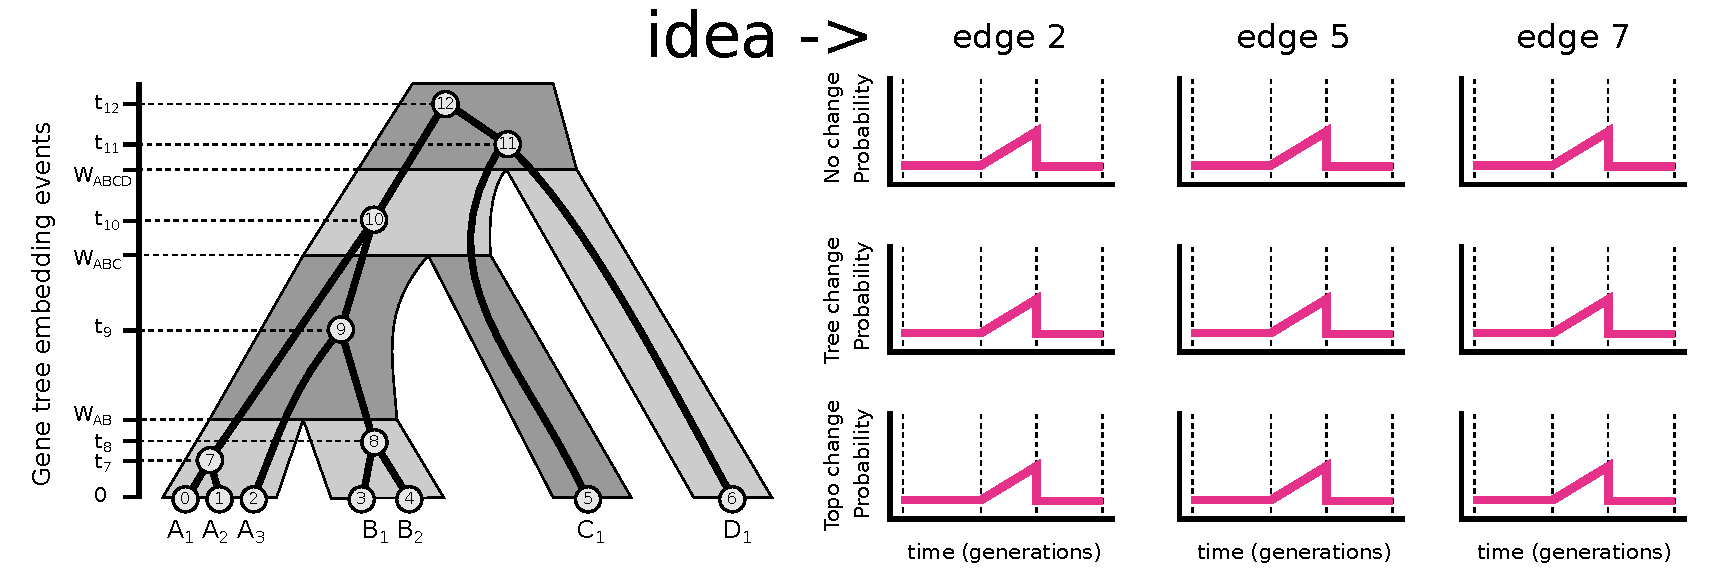
\includegraphics[width=0.99\textwidth]{figures/Fig3-parameters-extend.pdf}
	\caption{A gene tree embedded in a species tree. 
	(a) Species tree divergence times ($W$) separate
	intervals, each of which can have different effective population sizes ($N_b$),
	which determine rates of coalescence in each interval. Viewed backwards in time, 
	coalescent events (e.g., $t_7$) reduce the number of samples, whereas species tree
	divergence events (e.g., $W_{AB}$) increase the number of samples present. 
	(b-d) Recombination is modeled by detaching a branch at a specific time and 
	sampling a waiting time until it re-coalesces, leading to either no change, 
	a tree change (edge lengths), or topology change. Edges 2, 5, and 7 span multiple
	intervals where coalescent rates change, leading to different probabilities of
	outcomes (discussed in text). See Table 1 for the full gene tree embedding table.
	}
	\label{fig:fig1}
\end{figure}


Importantly, both the coalescent and MSC are models of the expected distribution of 
\emph{unlinked} (uncorrelated) genealogies.
%(non-autocorrelated) genealogies. % sampled from throughout the genome. 
By contrast, two linked genealogies that are drawn from nearby regions of a genome %the genome 
are expected to be more similar than two random draws under these models. This spatial 
autocorrelation is a consequence of shared ancestry among samples at nearby regions, 
which decays over time and distance as recombination events reduce their shared ancestry.
This process can be approximated by randomly breaking an edge on a genealogy and sampling
a waiting time (based on the lineage effective population size) until it reconnects
to the genealogy at a different shared ancestor (Fig.~\ref{fig:fig2}). 
In this way, the coalescent with recombination can be viewed as a process 
where a set of samples at the present substitutes one ancestor for another on 
either side of a recombination breakpoint. 
% \citep{wiuf_recombination_1999}. 


An algorithm to simulate the coalescent with recombination was developed early
on \citep{hudson1983properties},
% , however only with recent advances has it become 
% tractable to scale such simulations to larger, genome-wide scales 
% \citep{kelleher2016efficient}. 
% former new paragraph
% Although it is relatively simple to simulate the coalescent with recombination it has
% proven more challenging to develop an analytical solution for its expected outcome. 
however it has since proven more challenging to develop an analytical solution for 
its expected outcome. 
This includes 
% the a inference of 
%coalescent times on 
\hl{a distribution of linked } 
genealogies as well as the 
% distribution of 
breakpoints across the genome where recombination occurred 
(i.e., "waiting distances" between genealogies).
As a data structure,
this can be represented either as an ancestral recombination graph (ARG)
\citep{griffiths_ancestral_1996} or tree-sequence \citep{kelleher2016efficient}
(hereafter we will refer to it as an ARG).
% (we will refer to ARGs hereafter; Fig. S1).
% While our ability to simulate the coalescent with recombination has made substantial progress, likelihood-based inference of recombination events and coalescent times (that is, the ancestral recombination graph -- "ARG") is notoriously difficult \citep{griffiths_ancestral_1996}. 
% Unfortunately, 
Inference of ARGs is computationally intensive, highly limited by 
sequence information, and can be nearly infinite in possibilities for large 
genome lengths and numbers of samples \citep{mcvean2005approximating}. 
% In other words, there
% are usually very few mutations to provide information about each genealogy, 
% and ...
A major advance was achieved through development of the Sequentially Markov 
Coalescent (SMC), a simplification of the space of possible ARGs that 
restricts the types of coalescent events that can occur between sequential
genealogies, in a way that enables modeling
% models 
% changes among sequential genealogies 
them as a Markov process 
\citep{mcvean2005approximating}. 
Implicit to SMC-based methods is the expectation that recombination occurs at 
some rate from which the waiting distance between recombination events can be modeled 
as an exponentially distributed random variable. 
Under these assumptions a tractable likelihood framework can be developed. 
% inferring modeling
% The SMC provides a generative framework for producing a set of genealogies
% and segment lengths under a set of rules 
% The SMC (and related methods) provides a likelihood function 
% for the probability of observing a sequence of genealogies 
% pairwise coalescence times 
% and corresponding segment lengths between them on a genome, 
% given an effective population size and recombination rate. 
% 
% provides a generative framework for genealogies and segment lenghts under 
% a set of rules on which likelihood inference methods can be developed...
% 
% NEXT< start with Because, or something, not however,... 'this is how it is implemented in hmms'
% However, 
Because both genealogies and segment lengths cannot
be observed directly, most SMC-based methods use 
% employ 
hidden Markov model (HMM) methods to treat these as hidden states to
be inferred from sequence data. 
% he segment lengths and coalescent times are unknown, most methods use hidden Markov 
% model (HMM) methods in which these are hidden states inferred from sequence 
% data. 
% Further extensions have been developed for modeling variable 
Examples include tools for inferring changes in effective population 
sizes through time of single (PSMC) or multiple populations (MSMC) 
based on pairwise coalescent times \citep{li2011inference, schiffels_inferring_2014}, 
as well as methods for inferring ARGs using SMC-based conditional 
sampling methods
% based on SMC-like simulations
\citep[ARGweaver;][]{rasmussen2014genome, hubisz2020inference}.


% –- using an approach similar to 
% algorithms for simulating the coalescent with recombination –- 

% However, by modeling the coalescent with recombination
% using a Markovian approximation called the Sequentially Markov Coalescent (SMC), ARG 
% inference becomes more tractable.   
% The SMC is a simplification of the space of possible ARGs -- using an approach similar 
% to the algorithms for simulating the coalescent with recombination -- that models changes
% among sequential genealogies as a Markov process \citep{mcvean2005approximating}.
% IS THIS TECHNICALLY CORRECT?
% \hl{Under the SMC, the likelihood of a sequential set of genealogies and recombination 
% breakpoints (i.e., an ARG) is computed as the product of the set of independent likelihoods
% of observing each change from one genealogy to the next, given an effective population size
% and recombination rate.}
% While explicit likelihood-based inference of ARGs is still difficult, the SMC has enabled 
% \hl{several heuristic approaches to estimating ARGs from sequence data based on inferred 
% recombination events and differences in coalescent times among linked genealogies}
% \citep{li2011inference,rasmussen2014genome,hubisz2020inference}.
% , and the similarities among sequential genealogies, to model
% changes in effective population sizes \citep{}, and to infer 
% ARGs from sequence data 
% historical inferences about changes in effective population sizes, 
% recombination rates, and selection 


% Is this paragraph important? Maybe move to discussion. Concatalescence is not super important to intro.
% Despite the many advances that have been developed for incorporating information 
% from recombination into coalescent inference, the MSC framework (and related 
% fields in phylogenetics, such as the network multispecies coalescent 
% \citep{degnan2018modeling}) continues to largely treat recombination as a source 
% of error as opposed to information.
% This stems from the widely known expectation that, in parts of parameter space, 
% concatenation of sequences from multiple distinct genealogical histories can mislead
% phylogenetic inference. If a concatenated sequence is used to infer a single tree
% representing the species relationships, it might converge on a topology that is different
% from the species tree topology \citep{degnan2006discordance,kubatko2007inconsistency}. 
% The same concatenation biases can affect the distribution of inferred gene trees at
% individual loci as well, with potential effects on species tree or network inference
% methods that take multiple gene trees as inputs -- a process termed "concatalescence"
% \citep{gatesy_concatenation_2013}. The extent to which genetic loci (e.g., exons, UCEs,
% genome windows) represent a single versus multiple genealogical histories can be 
% estimated with coalescent simulations under an MSC model with recombination 
% \citep{mckenzie2020multispecies}. However, analytical solutions have not been
% developed to describe these as distributions within a statistical phylogenetic framework. 


\begin{figure}
	\centering
	%\fbox{\rule[-.5cm]{4cm}{4cm} \rule[-.5cm]{4cm}{0cm}}
	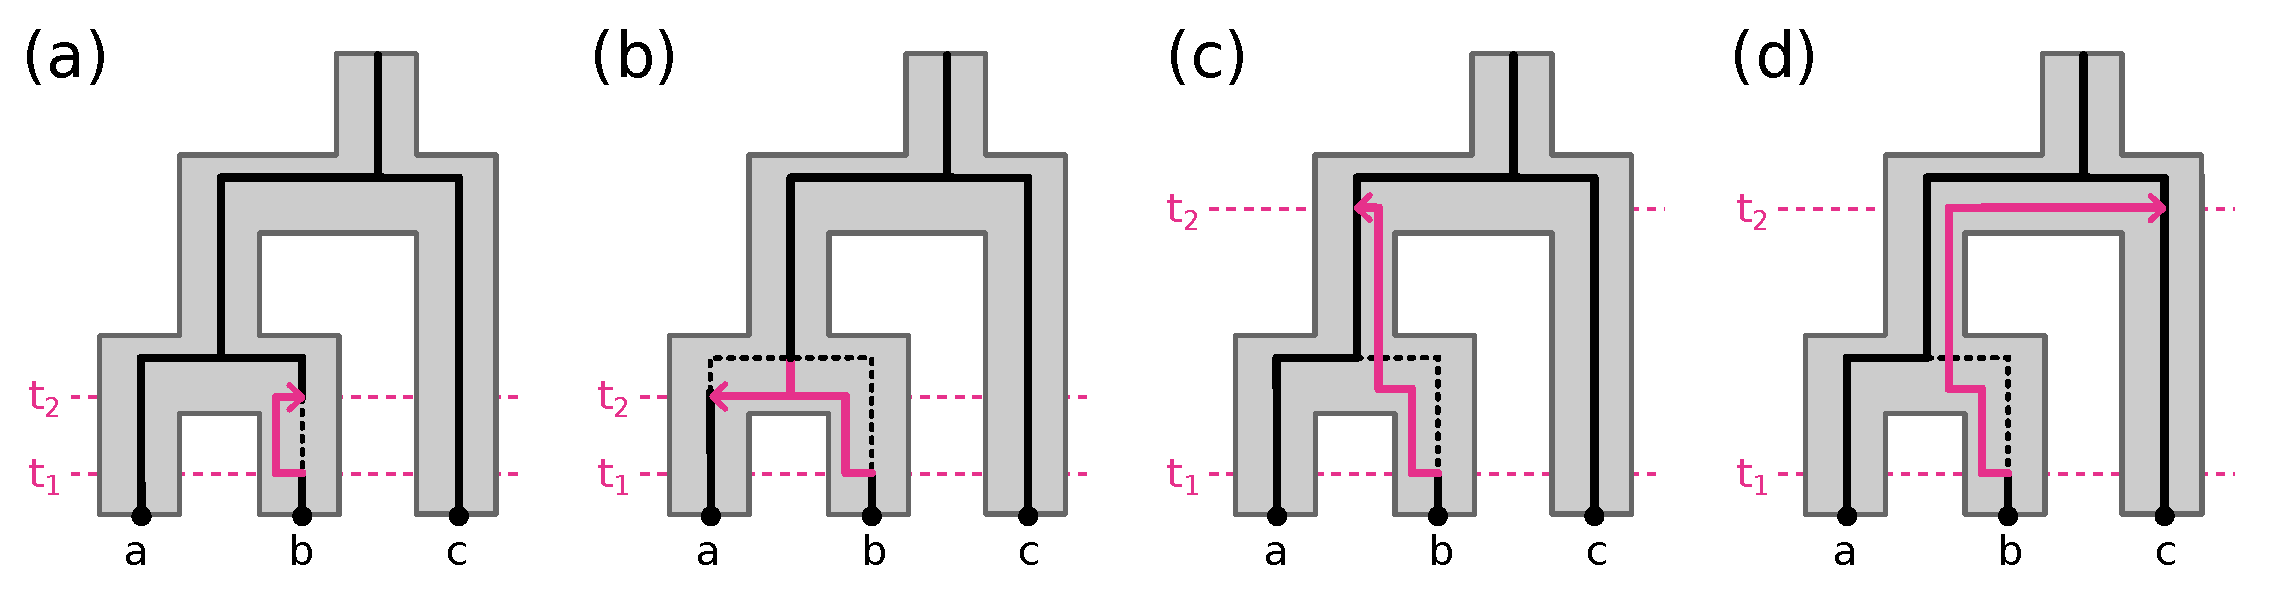
\includegraphics[width=0.9\textwidth]{figures/Fig2-new-recomb-types.pdf}
	\caption{
	Examples of the four different categories of outcomes from a 
	recombination event (adapted from \citep{deng_distribution_2021}). 
	(a) A category 1 event occurs when the dislocated lineage reattaches to the 
	original lineage. 
	(b) A category 2 event occurs when a dislocated lineage attaches to its 
	sibling lineage (the lineage that it originally coalesced with), shortening 
	both of their branch lengths and extending that of its parental lineage. 
	(c) A category 3 event occurs when the dislocated lineage attaches to its 
	parental lineage, lengthening the original lineage and its sibling lineage,
	and shortening the parental lineage.
	(d) A category 4 recombination event occurs when the dislocated lineage
	attaches with any lineage other than itself, its sibling lineage, and its
	parental lineage. This is the only category of recombination event that
	changes the topology of the genealogy.
}
\label{fig:fig2}
\end{figure}


% Implicit to SMC-based methods is the expectation that recombination occurs at 
% some rate from which the waiting distance between recombination events can be modeled 
% as an exponentially distributed random variable. 
\cite{marjoram2006fast}
described an important extension to the SMC, termed the SMC', for additionally
modeling "invisible" recombination events that result in no change between 
neighboring genealogies, which has been shown to significantly improve SMC-based 
inferences \citep{wilton2015smc}. Under the SMC', there are thus four categories
of possible outcomes of recombination (Fig.~\ref{fig:fig2}): 
(1) no change between sequential genealogies;
(2) shortening of a coalescent time; (3) lengthening of a coalescent time; 
and (4) a coalescent event that changes the topology (relationships). 
These can be grouped more generally into three categories: 
"no change" (type 1), "tree change" (types 2 or 3), and "topology change"
(type 4). Recently, \citet{deng_distribution_2021} derived a set of solutions for
the expected waiting distances between these three categories of 
outcomes for a single population with constant effective population size.
% Although all three outcomes, and their associated waiting distances, occur 
% implicitly between sequential genealogies within data generated under the SMC', 
% there was not previously a solution for expectations between events that do 
% not occur sequentially, representing the joint probabilities of multiple events.
% This provides an important advance, for establishing a neutral expectation for 
% turnover 
% in different categorical types of genealogy changes, and for connecting these
% to coalescent model parameters, which may prove useful for future ARG inference 
% tools. 
This provides an important advance in establishing a neutral expectation not
only for a generic recombination events to occur, but for different types 
of events that leave different detectable signatures in the genome.
% ,which may prove useful for the development of future SMC'-based tools.
% in genealogical topologies, and for connecting coalescent model parameters to these
% outcomes, which may prove useful for future advances in ARG inference. 

% \citep{deng_distribution_2021} recently 
% Their solution assumes a single population with constant effective population size, 
% but nevertheless ... 
% Their solutions 


% recently described a partitioning of different possible outcomes of recombination 
% events into three categories: (1) "no effect", which do not change the genealogy; 
% (2) "tree changes", which affect only coalescent times (edge lengths); and 
% (3) "topology changes", which affect the genealogical relationships.

% the expected waiting distances between
% recombination events, describing different rates for three categorical
% types of recombination events that can occur (Fig.~\ref{fig:fig2}). 
% % 
% This includes recombination events that: (1) have no affect on the 
% genealogical tree; (2) cause "tree changes" (i.e. that they 
% affect either the branch lengths or the topology of the genealogical tree, 
% as in any of categories 2, 3, and 4), and those that cause "topology changes" 
% (only category 4) (\textbf{Figure 1}).


% \citet{deng_distribution_2021} derived an approximate solution for the 
% distribution of waiting distances between sequential genealogies in an ARG. 
% This involved extending the simple expectation for the expected waiting distance
% between *any* recombination event, and partitioning the results into categories
% of different possible outcomes (Fig.~\ref{fig:fig2}). 

% , some of which result in changes to 
% the genealogy, and others of which do not. 
% This represents a major advance. Although 
% The expected waiting distance between any recombination event can be modeled as
% a simple simply described by an exponential distribution}, 
 % under the SMC’ 

% an extension of the SMC that includes "invisible" recombination
% events that result in no change between neighboring genealogical trees. 
% \hl{was known previously}, 
% \citet{deng_distribution_2021} 


Here, we extend the methods of \citet{deng_distribution_2021} to an MSC framework
to approximate the expected waiting distances between different categories of 
genealogy changes under a parameterized species tree model. In this respect, 
the waiting distances between recombination events of type 4 may be of greatest 
interest, as topology changes leave the most detectable signatures in sequence data, 
and are relevant to expected gene tree distributions that form an important 
component of many MSC-based methods.
However, events of types 1-3 \hl{are also interesting,} as they may occur 
disproportionately often in small sample sizes \citep{wilton2015smc}, 
which are especially common in MSC-type datasets, where
samples are partitioned among species tree intervals. The partitioning of 
coalescent events among species tree intervals is thus expected to constrain 
the types of recombination events that will be observed. Consequently, the
distributions of waiting distances between different categories of 
genealogy changes should be highly dependent on, and thus informative about, 
the species tree model. We refer to this general framework of embedding the 
SMC' in an MSC model as the MS-SMC.


% The relative frequency
% of different event types is therefore expected to be contingent on parameters
% of the species tree. 

% Recombination events of type 4 are of greatest interest
% % the most inherently interesting 
% for most applications,
% % because s
% as they leave the most detectable signal in sequence data.
% % since they will produce the most obvious signal in the sequence data. 
% However, events of types 1-3 occur disproportionately often in small sample 
% sizes \citep{wilton2015smc}, which are especially common in MSC-based studies, 
% where genealogies are embedded within a species tree, such that fewer samples 
% typically represent each lineage. But the
% relative frequency of the different events is contingent upon the Ne values of the
% species tree branches and on the species divergence times. In other words, the 
% partitioning of coalescence events among lineages of the species tree topology is
% expected to constrain the types of recombination events that are more likely to be
% observed. This results in distributions of waiting distances between genealogical
% changes being highly dependent upon parameters of the species tree model. 

% With this in mind, we extend the method of \citet{deng_distribution_2021} to the MSC
% to predict the expected waiting distances between genealogy changes under a 
% parameterized species tree model. This new solution is important for establishing an 
% expectation for the neutral rate of genealogy turnover under different species tree 
% parameterizations. It may also have applications for ARG inference under complex 
% demographic models \citep[e.g.,][]{hubisz2020mapping}, potentially serving as a 
% component of a likelihood function for inferring species trees from linked 
% genealogies -- a future theoretical goal.

% MS-SMC: multispecies sequentially markovian coalescent
% SM-MSC: sequentially markovian multispecies coalescent

%Solutions exist for simulating genomes under the coalescent with recombination \citet{ipcoal, kelleher, hudson}. In particular, \emph{msprime} is a powerful and flexible tool for simulating ancestral recombination graphs for many samples under user-defined demographic scenarios. \emph{ipcoal} is an extension of msprime that accepts multispecies coalescent parameters. 

%Phylogenetic methods sampling regions throughout the genome have increasingly adopted the multispecies coalescent model to incorporate variation in regions due to incomplete lineage sorting. Applications of the multispecies coalescent in phylogenetic inference aim to avoid known bias under which, in certain circumstances, phylogenies inferred from concatenated data might converge on a tree that is not the species tree. One challenge of applying the multispecies coalescent for species tree inference is properly defining the breakpoints for loci used in the analysis. Often this is done arbitrarily: researchers ensure that loci are long enough to infer reliable gene trees, and that there are enough inferred gene trees to infer a robust species tree. However, there has been some debate in the literature over the effects of locus length on species tree inference. Specifically,  

%Another way in which the ancestral recombination graph is relevant to phylogeneticists is for local inference...

%Recently, \citet{deng_distribution_2021} provided a solution for the distribution of waiting times to genealogical changes under the SMC', a popular model for simulating ancestral recombination graphs. However, their solution is constrained to a single population of constant effective population size.

%Establishing the predicted length of different topologies along the chromosome is important for inference of local genealogies in population genetics, which can be used for inference of selection, demographic changes, and introgression. It is also important in multispecies coalescent methods in phylogenetics, which often rely on inference of gene trees.


% springer + gatesy

% inference, argweaver-D

\section{Approach}
\subsection{Comparison to \citet{deng_distribution_2021}}

Our approach is a generalization of the \citet{deng_distribution_2021} derivation 
of waiting distances to genealogy changes for a single population of constant size. 
We modified the single-population model to (1) include barriers to coalescence imposed
by a species tree topology, and (2) integrate over changing coalescence rates along
paths through multiple species tree intervals with different effective population 
sizes. 
% I don't feel particularly inclined to follow their variables. I think it would be
% cleaner to translate it to cleaner variables to align better with MSC theory.
We have intentionally reproduced our equations in a similar structure and using
many of the same variable names as in \citet{deng_distribution_2021}.
% to highlight the changes we made to generalize their solution.

% \begin{figure}
% 	\centering
% 	%\fbox{\rule[-.5cm]{4cm}{4cm} \rule[-.5cm]{4cm}{0cm}}
% 	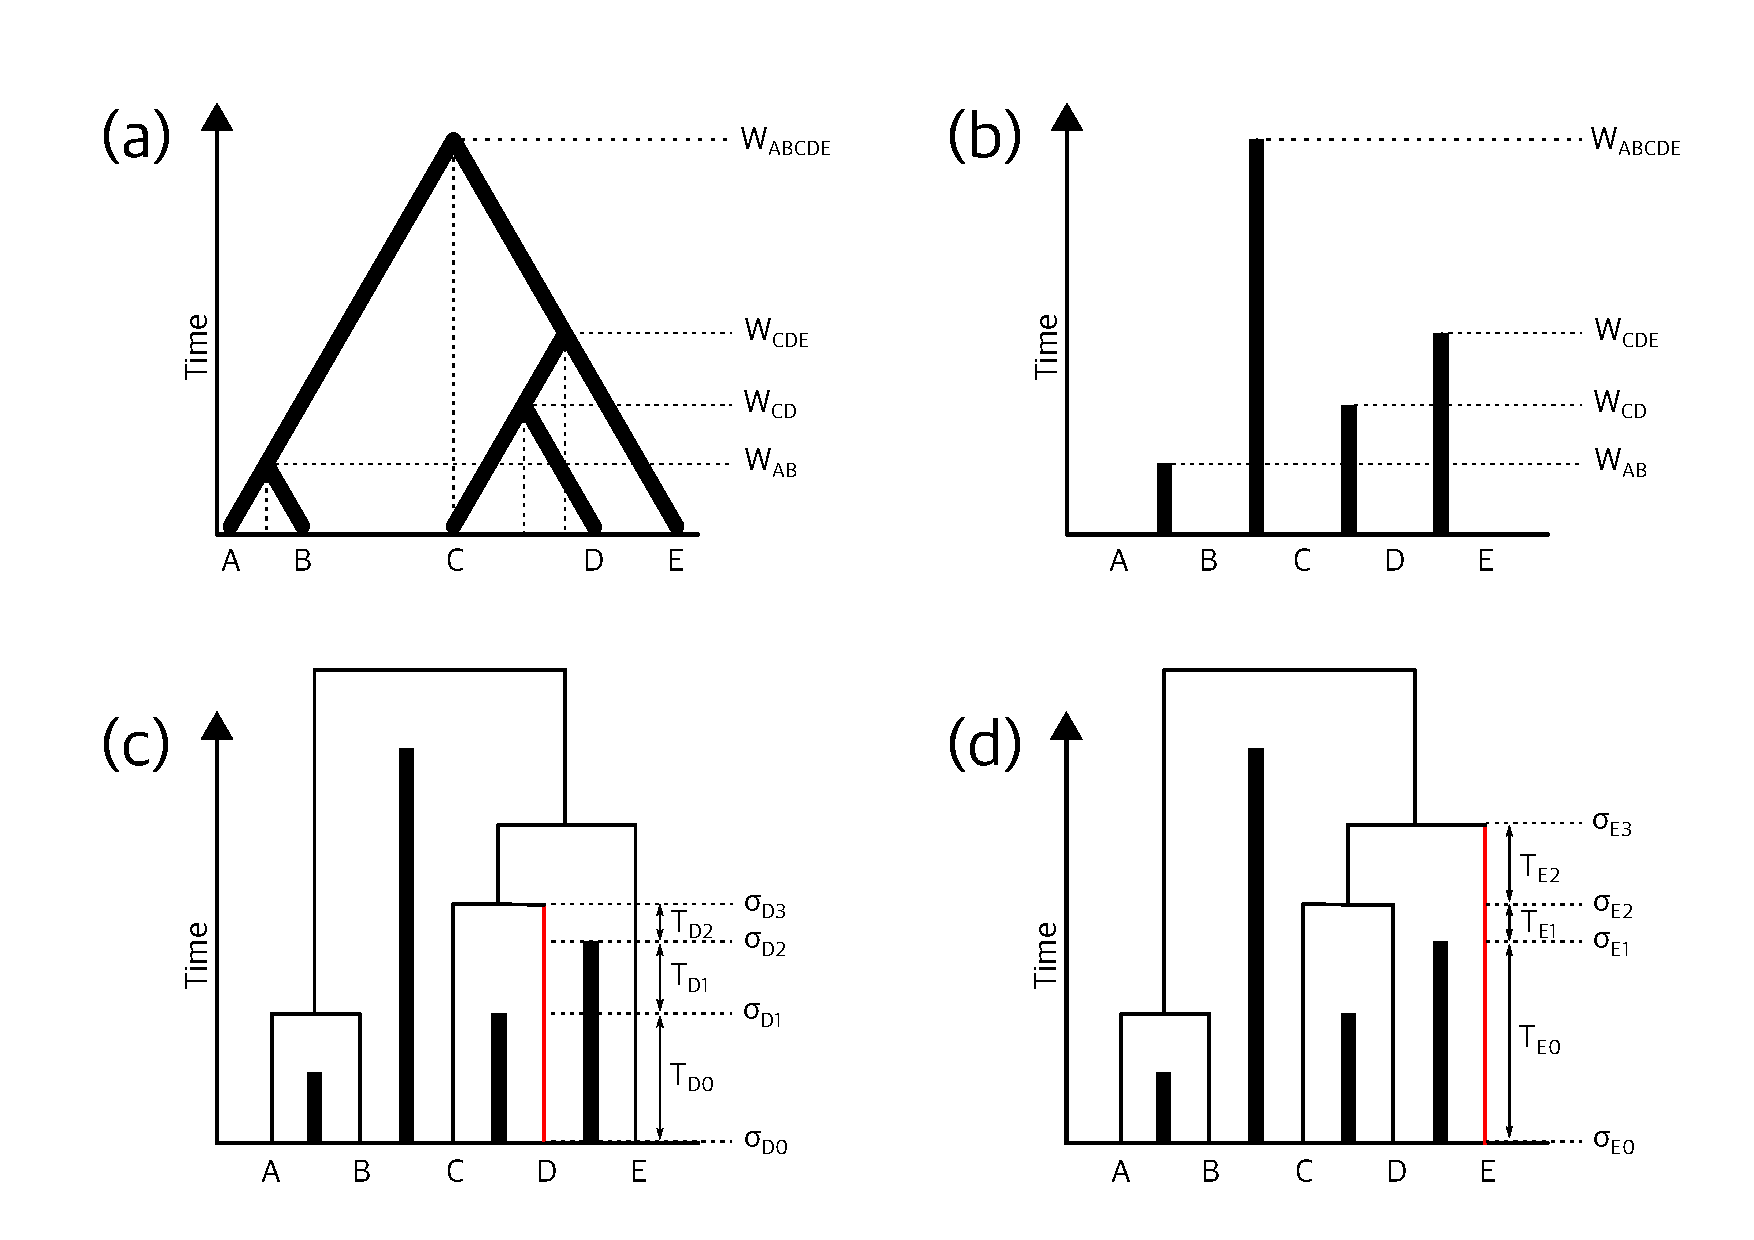
\includegraphics[width=0.9\textwidth]{figures/Fig3-panel-barriers.pdf}
% 	\caption{Illustrative depiction of the species tree model to introduce key parameters. a) A species tree topology with divergence times ($W$). Each branch has a characteristic effective population size (not shown). b) Alternative representation of the species tree that preserves topology and divergence times. This representation highlights how population divergences act as "walls" between populations, preventing coalescences between individuals from separate populations. c) A sampled genealogy embedded within the species tree, with focal branch D. The focal branch is broken into intervals with constant coalescence rates. The number of intervals in this branch, $\mathcal{I}_D$, is 3.  d) The same genealogy, but with focal branch E.}
% 	% \label{fig:fig1}
% \end{figure}



\subsection{MSC model description}
% We assume a species tree model with divergence times in units of generations and 
Given an MSC model composed of a species tree topology ($\mathcal{S}$), with divergence
times ($W$) in units of generations, and constant effective population sizes
assigned to each branch interval ($N_b$), a genealogy ($\mathcal{G}$) 
for any number of sampled gene copies can be generated by randomly sampling 
coalescent times %($t$) 
at which to join two samples into a common ancestor, 
starting from samples at the present in each interval. The rate of coalescence
is $\frac{1}{2N_b}$, and the expected waiting time between coalescence events
that will reduce the number of samples from $k$ to $k$-1 in a population 
follows the Kingman coalescent:

\begin{equation}
	\mathbb{E}(t_k| N_e) = \frac{k(k-1)}{2N_e}
\end{equation}

\noindent In a single population model
with constant $N_e$ this rate decreases monotonically as the number of remaining 
samples after each coalescence event decreases. In an MSC model, however, 
the rate of coalescence typically waxes and wanes through time, as the
transition from one branch interval to the next can be associated with 
different N$_b$ and an increase in $k$ as samples from 
descendant branch intervals are merged.

Based on this generative framework for sampling genealogies, a set of likelihood
solutions have been developed to fit coalescent model parameters, such as 
$N_e$ in single population models (\citep{kingman1982coalescent}), 
or $N_b$ and $W$ values in MSC 
models \citep{rannala2003bayes}, based on inferred coalescent times. 
In the latter framework, each species tree branch interval is treated independently, 
such that the likelihood of a genealogy embedding is calculated from the joint
probability of observing each distribution of coalescent waiting times within
each species tree branch interval. A key feature of these equations is that 
when $k$ lineages are present, we can use equation 1 as a rate parameter ($\lambda$)
to calculate the likelihood of an observed coalescent waiting time ($t_k$) between
$k$ and $k$-1 lineages from an exponential probability density:
% for the expected rate
% of coalescence
% between when $k$ and $k$ - 1 lineages exist. 
%  and thus the probability of 
% when Using the expected time between coalescence
% events when $k$ lineages are present (equation 1) as a rate parameter, the 
% likelihood of an observed waiting time can be calculated from an exponential 
% probability density. 
	
\begin{equation}
	% \mathcal{P}(t_k|\lambda) = \lambda e^{-\lambda t_k} 
	f(t_k) = \lambda e^{-\lambda t_k} 	
\end{equation}


% In each species tree interval this is repeated for each interval between 
% observed coalescent events.

% The probability of a particular genealogical topology among a set of coalesced
% samples in an interval. The probability a particular pair of lineages coalesce
% is 1 ( kchoose2) = (2 / (j * (j - 1))), where j=m, n, n+1. [Describe m and n as
% the start and end of intervals.]

% \begin{equation}
% 	\mathbb{P}(t_k | N_e) = 
% 		\frac{1}{2N_e} 
% 		\exp \bigg\{-\frac{k(k-1)}{4N_e} t_k \bigg\} \times 
% 		\exp \bigg\{-\frac{n(n-1)}{4N_e} (\tau - (t_m + t_{m-1} + \text{...} + t_{m+1})) \bigg\}
% \end{equation}

% Similarly, the likelihood of observing a set of coalescent
% times on a genealogy embedded in a species tree can be calculated from the
% joint probability of its observed coalescence times within each interval
% \citep{rannala2003bayes}, treating intervals independently. 
% Thus, the genealogy (G) in Figure 1 can be calculated as
% ...

% Generating unlinked genealogical trees under the MSC is straightforward: Coalescent events between samples can only happen after (moving backward in time) coalescence of the species that contain them, and the coalescent rate in each part of the tree is dependent on both the number of genealogical lineages that can coalesce in that section and on the effective population size in that section.

\subsection{MS-SMC' model description and notation}

% Under the single-population SMC' 
% considered by \citet{deng_distribution_2021}, the 
Under the SMC' model, sampling of a linked genealogy requires considering not only 
%a species tree and its parameters, 
coalescent model parameters, 
as we did above, but also an existing genealogy -- it is a method 
for sampling the next genealogy conditional on the previously observed one. 
If we define the previous genealogy as $\mathcal{G}$, and the sum of its edge lengths 
as $L(\mathcal{G})$, then under the assumption of a constant recombination rate through time,
a recombination break point can be uniformly sampled from $L(\mathcal{G})$ to occur with 
equal probability anywhere on $\mathcal{G}$. A recombination event creates 
a bisection on an edge, separating a subtree below the cut from the rest of 
the genealogy (Fig.~\ref{fig:fig2}). The subtree must then be reconnected by sampling a new common 
ancestor between it and the other samples still connected to the genealogy, which 
must occur above the time of the cut. This re-connection point is sampled 
probabilistically with an expected waiting time until re-coalescence the 
same as described above (equations 1 and 2).

In a single population model with constant N$_e$ the re-coalescent probability
after a recombination event decreases monotonically, as each subsequent 
coalescence event decreases $k$.
% (e.g., Fig.~1B). 
Once again, the MSC model 
differs from this: coalescent events similarly decrease $k$, but the merging of 
species tree branches into ancestral intervals increases $k$, and effective population 
sizes can also vary among species tree intervals. 
Thus, the probability that a subtree re-connects to the genealogy can vary 
along its path of possible reconnection points through 
different species tree intervals.
% (Fig.~1C). 
A species tree can thus be decomposed into a series of relevant intervals 
between events that change the rate of coalescence
% , including within species tree intervals, 
which we refer to as the gene tree embedding 
table (Table~\ref{tab:table-1}). 

Each branch ($b$) of $\mathcal{G}$ spans one or more intervals
from which a lower and upper (min, max) bound for that 
edge can also be extracted ($t_b^l$ and $t_b^u$, respectively). 
The time of the start of each interval ($i$) is $\sigma_i$. 
An integer index ($\mathcal{I}$) stores the number of intervals that 
each branch occurs in, such that enumerating over the range
of ($\mathcal{I}$) can visit each interval of a genealogy branch.
% . For example, 
% edge 2 from Fig.~\ref{fig:fig1} and Table~\ref{tab:table-1} overlaps with 
% three intervals, such that $\mathcal{I}_2$ = 3.
% \hl{From this gene tree embedding we also define 
% the set $\mathcal{I}$ that includes the indices of all intervals in the table. 
% And we define an indexing variable $I_b$ for each branch ($b$) in $\mathcal{G}$ that
% returns a vector of ordered intervals ($i \in \mathcal{I}$) that overlap with 
% a specific gene tree branch.}
% For example, edge 2 from Fig.~\ref{fig:fig1} and Table~\ref{tab:table-1} overlaps with 
% three intervals, such that $I_2$ = (0, 1, 6). 
These variables,
and the gene tree embedding table, includes all relevant parameters
for the derivations below.
% , and are also summarized in the Appendix.

\hl{needs updates to figure out how table can align with existing variables names.
Additional table with final info could be supplement. Includes I, sister index, parent index...}

% Unlike in the single-population SMC', the intervals in the multispecies model
% are branch-specific. For example, the breakpoint $\sigma_{D1}$ in Figure 2c  
% corresponds to the species tree coalescence of species C and species D. This 
% increases the number of lineages available for the D lineage to coalesce with 
% (from 1 -- itself -- to 2) and might also change the effective population size.
% However, this breakpoint does not appear in Figure 2d since the lineage in species
% E is not able to coalesce with lineages from species C or D until $\sigma_{E1}$,
% when E coalesces with the ancestor of C and D in the species tree.


\begin{table}[h]
\centering
\caption{\label{tab:table-1} 
	A gene tree embedding table for MS-SMC' calculations for the gene tree and
 	species tree in Figure 1. 
	% Coalescent waiting times in each interval can be calculated from the number of lineages
	% present ($k$) and the effective population size ($N_e$). 
	% To integrate over the probability of coalescence on a specific gene tree edge 
	% (e.g., edge 2 from Figure 1), involves integrating over all intervals that include 
	% that gene tree edge (e.g., rows 0, 1, and 6 for gene tree edge 2).
}
\begin{tabular}[t]{ |c|c|c|c|c|c|c|c|c| }
	\toprule
	 & start ($t_i^l$)  & end ($t_i^u$) & pop & $N_e$ ($n_i$)  & N edges ($a_i$) & coal  & length ($d_i$) & branches \\
	\midrule
	0 & 0          & $t_7$      & A   & $N_A$     & 3 & $t_7$    & $t_7$ - 0            & 0,1,2 \\
	1 & $t_7$      & $W_{AB}$   & A   & $N_A$     & 2 & -        & $W_{AB}$ - $t_7$     & 2,7   \\	
	2 & 0          & $t_8$      & B   & $N_B$     & 2 & $t_8$    & $t_8$ - 0            & 3,4   \\ 
	3 & $t_8$      & $W_{AB}$   & B   & $N_B$     & 1 & -        & $W_{AB}$ - $t_8$     & 8     \\
	4 & 0          & $W_{ABC}$  & C   & $N_C$     & 1 & -        & $W_{ABC}$            & 5     \\
	5 & 0          & $W_{ABCD}$ & D   & $N_D$     & 1 & -        & $W_{ABCD}$           & 6     \\
	% 
	6 & $W_{AB}$   & $t_9$      & AB  & $N_{AB}$  & 3 & $t_9$    & $t_9$ - $W_{AB}$     & 2,7,8 \\
	7 & $t_9$      & $W_{ABC}$  & AB  & $N_{AB}$  & 2 & -        & $W_{ABC}$ - $t_9$    & 7,9   \\
	% 
	8 & $W_{ABC}$  & $t_{10}$   & ABC & $N_{ABC}$ & 3 & $t_{10}$ & $t_{10}$ - $W_{ABC}$ & 5,7,9  \\
	9 & $t_{10}$   & $W_{ABCD}$ & ABC & $N_{ABC}$ & 2 & -        & $W_{ABCD}$ - $t_{10}$ & 5,10 \\
	%
	10 & $W_{ABCD}$ & $t_{11}$  & ABCD & $N_{ABCD}$ & 3 & $t_{11}$ & $t_{11}$ - $W_{ABCD}$ & 5,6,10 \\
	11 & $t_{11}$  & $t_{12}$   & ABCD & $N_{ABCD}$ & 2 & $t_{12}$ & $t_{12}$ - $t_{11}$ & 10,11 \\
	12 & $t_{12}$  & -          & ABCD & $N_{ABCD}$ & 1 & -        & -                   & 12    \\	
	\bottomrule
\end{tabular}
\end{table}



% In the MS-SMC', we specify a model with piecewise-constant coalescence rates. 
% However, intervals under the MSC adaptation are bounded not just by coalescence
% events in the \emph{genealogy} tree (decreasing the number of available lineages for 
% coalescence), but also by relevant coalescences in the \emph{species} tree. Species 
% coalesence events increase the number of genealogical lineages available for 
% coalescence, and they also can correspond to changes in effective population 
% size (\textbf{Figure 2}). 

% Having described our model, we also adopt the following notation:

% \begin{itemize}
%   \item $\mathcal{I}_b$: index of an interval on genealogy branch $b$. A genealogy 
%   branch is split into discrete intervals corresponding to points along its length 
%   at which either the species tree interval changes, or the number of samples $k$ with
%   which it can coalesce changes.
%   \item $t^u_b$: the height, in generations, of the upper bound of genealogy branch $b$.
%   \item $t^l_b$: the height, in generations, of the lower bound of genealogy branch $b$.
%   \item $\mathcal{T}$: the genealogical tree
%   \item $\mathcal{S}$: the species tree
%   \item $\mathcal{N}$: the number of tips in the species tree
%   \item $L(\mathcal{T})$: the total genealogical tree length, in generations
%   \item All summations where the stopping value is less than the starting value are equal to zero.
% \end{itemize}

% Several values are indicated only on one branch at a time, and thus we do not include 
% an underscore to indicate which branch. These are:
% \begin{itemize}
%   \item $\sigma_i$: the length, in generations, of the lower bound of interval $i$ on branch $b$.
%   \item $n_i$: the effective population size of species tree interval index $i$.
%   \item $a_i$: the number of available lineages to coalesce with in the genealogy interval with index $i$.
%   \item $T_i$: the length, in generations, of species tree interval with index $i$.
% \end{itemize}


\subsection{Deriving probabilities of genealogical changes in the MS-SMC}
A recombination can result in one of four categories of outcomes (Fig.~\ref{fig:fig2}), 
resulting in either no change to the genealogy, a change only to its branch lengths, 
or a change to its topology. Our first step in deriving probability statements for
these different outcomes is to calculate the probability of no change. Then, from
the law of total probability we can calculate probabilities of changes that 
% waiting distances to changes that 
fall into the other categories.
% In category 1, there is no change to the genealogy. In categories 2 and 3 only
% a the branch lengths of the genealogical tree change while the topology remains
% the same. In category 4, the topology of the resulting tree is different from the 
% original tree. For simplicity, we will refer to changes that affect only branch
% lengths (categories 2-3) as those that change \emph{the tree}, and category 4 as 
% those that change \emph{the topology}.
% Our first steps are to calculate the probability of a recombination event in
% category 1, where the new genealogical tree is identical to the previous tree. The 
% law of total probability then allows us to use the inverse probability to calculate
% a waiting distance to a change that falls into any of categories 2, 3, or 4. 

\subsubsection{Probability $t_r$ on branch $b$ does not change the tree:}
% \subsubsection{Probability that a recombination event at time $t$ on branch $b$ will not change the tree:}
% \hl{these sections needs waay more description. What does this all mean? The text here
% was only restating the section title. You need to build up to the more complex ones by 
% walking the readers through the more simple examples. I think this is super important
% to make this work understandable. Think of Rannala and Yang 2003.}
We begin by assuming knowledge of when and where recombination takes place, in terms 
of a recombination event bisecting branch $b$ at time $t_r$. The variable $\sigma$ 
The index $i$ indicates the gene tree embedding interval in which recombination occurs.
For no genealogy change to occur the detached branch must re-attach to its original 
lineage during the same interval in which it detached.
If it connects to any other existing lineages during this same interval, 
or coalesces in a later interval, this would lead to a change in either the 
tree or topology. A derivation of this equation can be found in the Appendix.
The first term corresponds to detaching from the focal interval and 
re-connecting to the same branch within it (i.e., $ii$), whereas the 
second term concerns re-connecting in a different interval (i.e., $ij$).
% where $i$ is the interval index in which $t_r$ occurs. 
\begin{equation}
\begin{aligned}
	&\mathbb{P}(\text{tree unchanged} | \mathcal{S},\mathcal{G},b,t_r) = 
	\bigg(\frac{1}{a_i} +P_{ii} \exp \bigg\{\frac{a_i}{n_i}t_r\bigg\}\bigg) + 
	\sum_{j=i+1}^{\mathcal{I}_b - 1} P_{ij} \exp\bigg\{\frac{a_i}{n_i}t_r\bigg\} 
\end{aligned}
\end{equation}

\noindent This includes the following two terms that will appear again.

\begin{equation}
\begin{aligned}
	% &P_{ii} = - \frac{1}{a_i} \exp \bigg\{-\frac{a_i}{n_i}(t_i^u - t_r) \bigg\} 
	&P_{ii} = - \frac{1}{a_i} \exp \bigg\{-\frac{a_i}{n_i}\sigma_{i + 1} \bigg\} 	
\end{aligned}
\end{equation}

\begin{equation}
\begin{aligned}
	&P_{ij} = 
	\left( \frac{1}{a_j} (1 - \exp \bigg\{ -\frac{a_j}{n_j} d_j \bigg\} \right)
	\times
	\exp \bigg\{ -\frac{a_i}{n_i}\sigma_{i+1} - 
	\sum_{q=i+1}^{j-1} \frac{a_q}{n_q} d_q \bigg \}
\end{aligned}
\end{equation}


% \begin{equation}
% \begin{aligned}
% 	&\mathbb{P}(\textrm{tree unchanged} | b,t,\mathcal{T},\mathcal{S}) = \frac{1}{a_i} +P_{ii}e^{\frac{a_i}{n_i}t}+ \sum_{k=i+1}^{\mathcal{I}_b-1} e^{\frac{a_i}{n_i}t} P_{ik}, \\
% 	&\text{where} \\
% 	&P_{ii} = - \frac{1}{a_i}e^{-\frac{a_i}{n_i}\sigma_{i+1}}, \\
% 	&\text{and} \\
% 	&P_{ik} = \exp\left(-\frac{a_i}{n_i}\sigma_{i+1}-\sum_{q=i+1}^{k-1} \frac{a_q}{n_q}T_q\right)\left(\frac{1}{a_{k}}(1-e^{-\frac{a_{k}}{n_{k}}T_{k}})\right),
% \end{aligned}
% \end{equation}

\subsubsection{Probability recombination on branch $b$ will not change the tree:}
By integrating the previous equation across all times at which recombination could
have occurred on branch $b$ (assuming a uniform recombination rate through time) 
we obtain the probability that recombination on this branch does not change the tree:

\begin{equation*}
	\mathbb{P}(\textrm{tree unchanged} | \mathcal{S}, \mathcal{G}, b) = 
	\frac{1}{t^u_b-t^l_b} \int_{t_b^l}^{t_b^u} 
	\mathbb{P}(\textrm{tree unchanged} | \mathcal{S},\mathcal{G},b,t)dt
\end{equation*}

\begin{equation}
	= \frac{1}{t^u_b - t^l_b}
	\sum_{i=0}^{\mathcal{I}_b-1} \frac{1}{a_i} d_i + 
	\frac{n_i}{a_i} 
	\bigg(
		\exp\bigg\{\frac{a_i}{n_i}\sigma_{i+1}\bigg\} - 
		\exp\bigg\{\frac{a_i}{n_i}\sigma_i\bigg\}
	\bigg)
	\bigg(\sum_{j=i}^{\mathcal{I}_b-1}P_{ij}\bigg)
\end{equation}


\subsubsection{Probability that a recombination event will not change the tree:}
Finally, by summing across all branches on the tree, while assuming a uniform 
recombination rate through time and across branches, we get the
probability that a recombination event will result in a category 1 outcome.

\begin{equation}
	\mathbb{P}(\textrm{tree unchanged} | \mathcal{S},\mathcal{G}) = 
	\sum_{b=1}^{2N-2}
	\left[\frac{t^u_b - t^l_b}{L(\mathcal{G})}\right]
	\mathbb{P}(\textrm{tree unchanged} | \mathcal{S},\mathcal{G},b)
\end{equation}

\noindent\hl{note: indexing branches from 1 instead of 0? is this consistent with other indexing?
Instead of numerically indexing 2N-2 (using another N variable) can be just say for all edges in G?
}

\subsubsection{Waiting distance to the next tree change:}
Under the SMC' the rate at which recombination events occur ($\lambda_r$)
is a product of the per-site per-generation recombination rate ($r$) and 
total branch lengths of the current genealogy.

\begin{equation}
	\lambda_{r} = L(\mathcal{G}) \times r
\end{equation}

\noindent And thus a waiting distance ($x$) to the next recombination event 
is distributed as an exponential probability density.

\begin{equation}
	f(x) = \lambda e^{-\lambda x}
\end{equation}

\noindent We can then modify this equation to instead yield probability
density for waiting distances to a recombination event that causes a 
tree change. 
Here, distances continue to be exponentially distributed, however, 
the new rate parameter ($\lambda_g$) is reduced proportionally by 
the probability that a recombination does not change the tree.

\begin{equation}
	\lambda_{g} = 
	L(\mathcal{G}) \times r \times 
	(1 - \mathbb{P}(\text{tree unchanged}|\mathcal{T},\mathcal{G}))
\end{equation}

% \begin{equation}
% \begin{aligned}
% 	&p_r(d|\mathcal{T},\mathcal{S}) = r\alpha_\mathcal{S}(\mathcal{T})L(\mathcal{T})\exp\left[-r\alpha_\mathcal{S}(\mathcal{T})L(\mathcal{T})d\right]\textrm{,} \\
% 	&where \\
% 	&\alpha_\mathcal{S}(\mathcal{T})=1-\mathbb{P}(\textrm{tree unchanged} | \mathcal{T},\mathcal{S})
% \end{aligned}
% \end{equation}

\subsection{Deriving probabilities of changes in the genealogical topology}

We can next derive an analogous probability density for the waiting distance 
to a change in the \emph{topology} of a genealogical tree. This involves excluding 
events of categories 2 and 3 to isolate the waiting distance to a category 4 event. 
Once again, we start with a branch-specific probability and then sum across all 
branches on the tree. In order to isolate tree changes that only affect edge
lengths from those that affect the topology we must take into account which 
specific branches the detached subtree from branch $b$ re-coalesces with. 
The two relevant branches are its sibling ($b'$) and parent ($c$). If it re-coalesces
with a sibling the topology remains the same but with a shortened 
coalescent time, and if it re-coalesces with its parent then its 
original coalescent time is simply lengthened. 
% The primary difference in this approach is that for any 
% branch $b$ we have to also consider coalescence possibilities with the branch above it 
% (branch $c$) and the branch with which it coalesces (branch $b'$). 
When labeling interval indices, we continue up branch $c$ so that the final index 
is equal to $\mathcal{I}_{b+c}-1$. 

We also introduce a new variable, $t_b^m$, which corresponds to the lowest point
at which branch $b$ can potentially coalesce with its sibling, branch $b'$. 
$t_b^m$ will always be the maximum of three values: the time at which $b$ and 
$b'$ are separated by a species divergence (if at all), the lowest point on 
branch $b'$ (i.e., $t_{b'}^l$), and $t_b^l$. We occasionally refer to interval
$m$, which is simply the interval whose lower bound is $t_b^m$.
\hl{this is relevant because ... elaborate maybe by referencing results figure}

\subsubsection{Probability that a recombination event on branch $b$ will not change the topology:}

We first present the probability that a recombination event occurring on a focal branch $b$ will change the tree topology. As in Section 2.3, this results from integrating through the solution when specifying a particular branch and time (see Appendix). 

\begin{equation}
\begin{aligned}
    &\mathbb{P}(\textrm{topology unchanged}|b, \mathcal{T},\mathcal{S}) = \frac{1}{t_b^u-t_b^l}\left[\sum_{i=0}^{m-1}p_{b,1}^{(i)}+\sum_{i=m}^{\mathcal{I}_b-1}p_{b,2}^{(i)}\right] \\
    &where: \\
    &p_{b,1}^{(i)} = \frac{1}{a_i}\left[T_i+n_i\left(\exp\left(\frac{a_i}{n_i}\sigma_{i+1}\right)-\exp\left(\frac{a_i}{n_i}\sigma_i\right)\right)\left(\sum_{k=i}^{\mathcal{I}_{b+c}-1}P_{ik}+\sum_{k=m}^{\mathcal{I}_b-1}P_{ik}\right)\right] \\
    &and: \\
    &p_{b,2}^{(i)} = \frac{1}{a_i}\left[2T_i + n_i\left(\exp\left(\frac{a_i}{n_i}\sigma_{i+1}\right)-\exp\left(\frac{a_i}{n_i}\sigma_{i}\right)\right)\left(2\sum_{k=i}^{\mathcal{I}_b-1}P_{ik}+\sum_{k=\mathcal{I}_b}^{\mathcal{I}_{b+c}-1}P_{ik}\right)\right]
    \end{aligned}
\end{equation}

\subsubsection{Probability that a recombination event will not change the topology:}

We simply sum the previous equation across all branches in the genealogy to 
determine the probability that a recombination event falling uniformly on the 
tree will change the topology.

\begin{equation*}
    \mathbb{P}(\textrm{topology unchanged}| \mathcal{T},\mathcal{S}) = \sum_{b=1}^{2N-2}\frac{t_b^u-t_b^l}{L(\mathcal{T})} \times \mathbb{P}(\textrm{topology unchanged}|b, \mathcal{T},\mathcal{S})
\end{equation*}

\begin{equation}
    = \frac{1}{L(\mathcal{T})}\sum_{b=1}^{2N-2}\left[\sum_{i=0}^{m-1}p_{b,1}^{(i)}+\sum_{i=m}^{\mathcal{I}_b-1}p_{b,2}^{(i)}\right]
\end{equation}

\subsubsection{Waiting distance to the next topology change:}

Unlike with the waiting distance to a \emph{tree} change, the exact waiting distance 
distribution to a change in \emph{topology} is complicated to derive because of 
possible intermediate recombination events that change the branch lengths but not 
the topology. These events impact the rate of recombination events and the probability
that each further recombination event changes the topology of the newly generated 
genealogy. However, \citet{deng_distribution_2021} demonstrate the approximate 
negation of this effect due to the inverse relationship between genealogy length
and the probability of a topology-changing recombination event. Even as branch 
lengths increase, reducing the waiting time to the next recombination event, the
probability that the recombination event will change the topology decreases. 
Therefore, we follow their approach by approximating the waiting distance to
a change in topology using an exponential distribution:
\noindent\hl{I suggest formulating this as a lambda value again, which makes it 
very clear how it is like the others.}

\begin{equation}
\begin{aligned}
	&p_r(d|\mathcal{T},\mathcal{S}) = r\beta_\mathcal{S}(\mathcal{T})L(\mathcal{T})\exp\left[-r\beta_\mathcal{S}(\mathcal{T})L(\mathcal{T})d\right]\textrm{,} \\
	&where \\
	&\beta_\mathcal{S}(\mathcal{T})=1-\mathbb{P}(\textrm{topology unchanged} | \mathcal{T},\mathcal{S}).
\end{aligned}
\end{equation}

\section{Demonstration}
% \label{sec:others}

We have implemented our solutions in the Python package \emph{ipcoal} 
\citep{mckenzie_ipcoal_2020}, which is an MSC-focused tool that includes
a wrapper around the coalescent simulation software \emph{msprime}
\citep{baumdicker_efficient_2022} paired with tree visualizations from
\emph{toytree} \citep{eaton_toytree_2020}. 
% Our MS-SMC functions are implemented in the subpackage \emph{ipcoal.smc}. 
Here we demonstrate
the accuracy of our solutions relative to simulated tree sequences.
Source code is available at \url{https://github.com/eaton-lab/ipcoal}
with reproducible examples implemented in jupyter notebooks.

% We adapted our solutions to python code, and we implemented them alongside the phylogenomic simulation package \emph{ipcoal} (an MSC-focused wrapper for the popular population genomic simulator \emph{msprime}) \citep{mckenzie_ipcoal_2020,baumdicker_efficient_2022}. Doing so facilitated three simple, illustrative analyses.

First, when given a species tree and initial genealogy, we could examine the probability of changes in the genealogy given a recombination event on a specific branch and at a specific time. \textbf{Figure 3} illustrates the selection of three branches from a genealogy embedded in a species tree model. The species tree was unbalanced with five tips, had equal internode distances of 2.5e5 generations, and had Ne of 2e5. Parts b, c, and d show the probability that a recombination event falling at each time on the 3 selected genealogy branches does not change the topology (i.e., the branch lengths might change, but the topology remains the same) and does not change the tree (i.e., both the branch lengths and topology remain unchanged). These results make clear that recombination events falling at the tops of branches (i.e., far right on the x-axis) are increasingly certain to change the branch lengths of the genealogy, since any re-coalescence of the detached branch can only occur above the recombination breakpoint. This also makes clear that recombination events occurring when there are only two lineages remaining are certain to not change the topology, since the two lineages are only able to re-coalesce with each other (as shown in the upper panels of c and d). 

\begin{figure}
	\centering
	%\fbox{\rule[-.5cm]{4cm}{4cm} \rule[-.5cm]{4cm}{0cm}}
	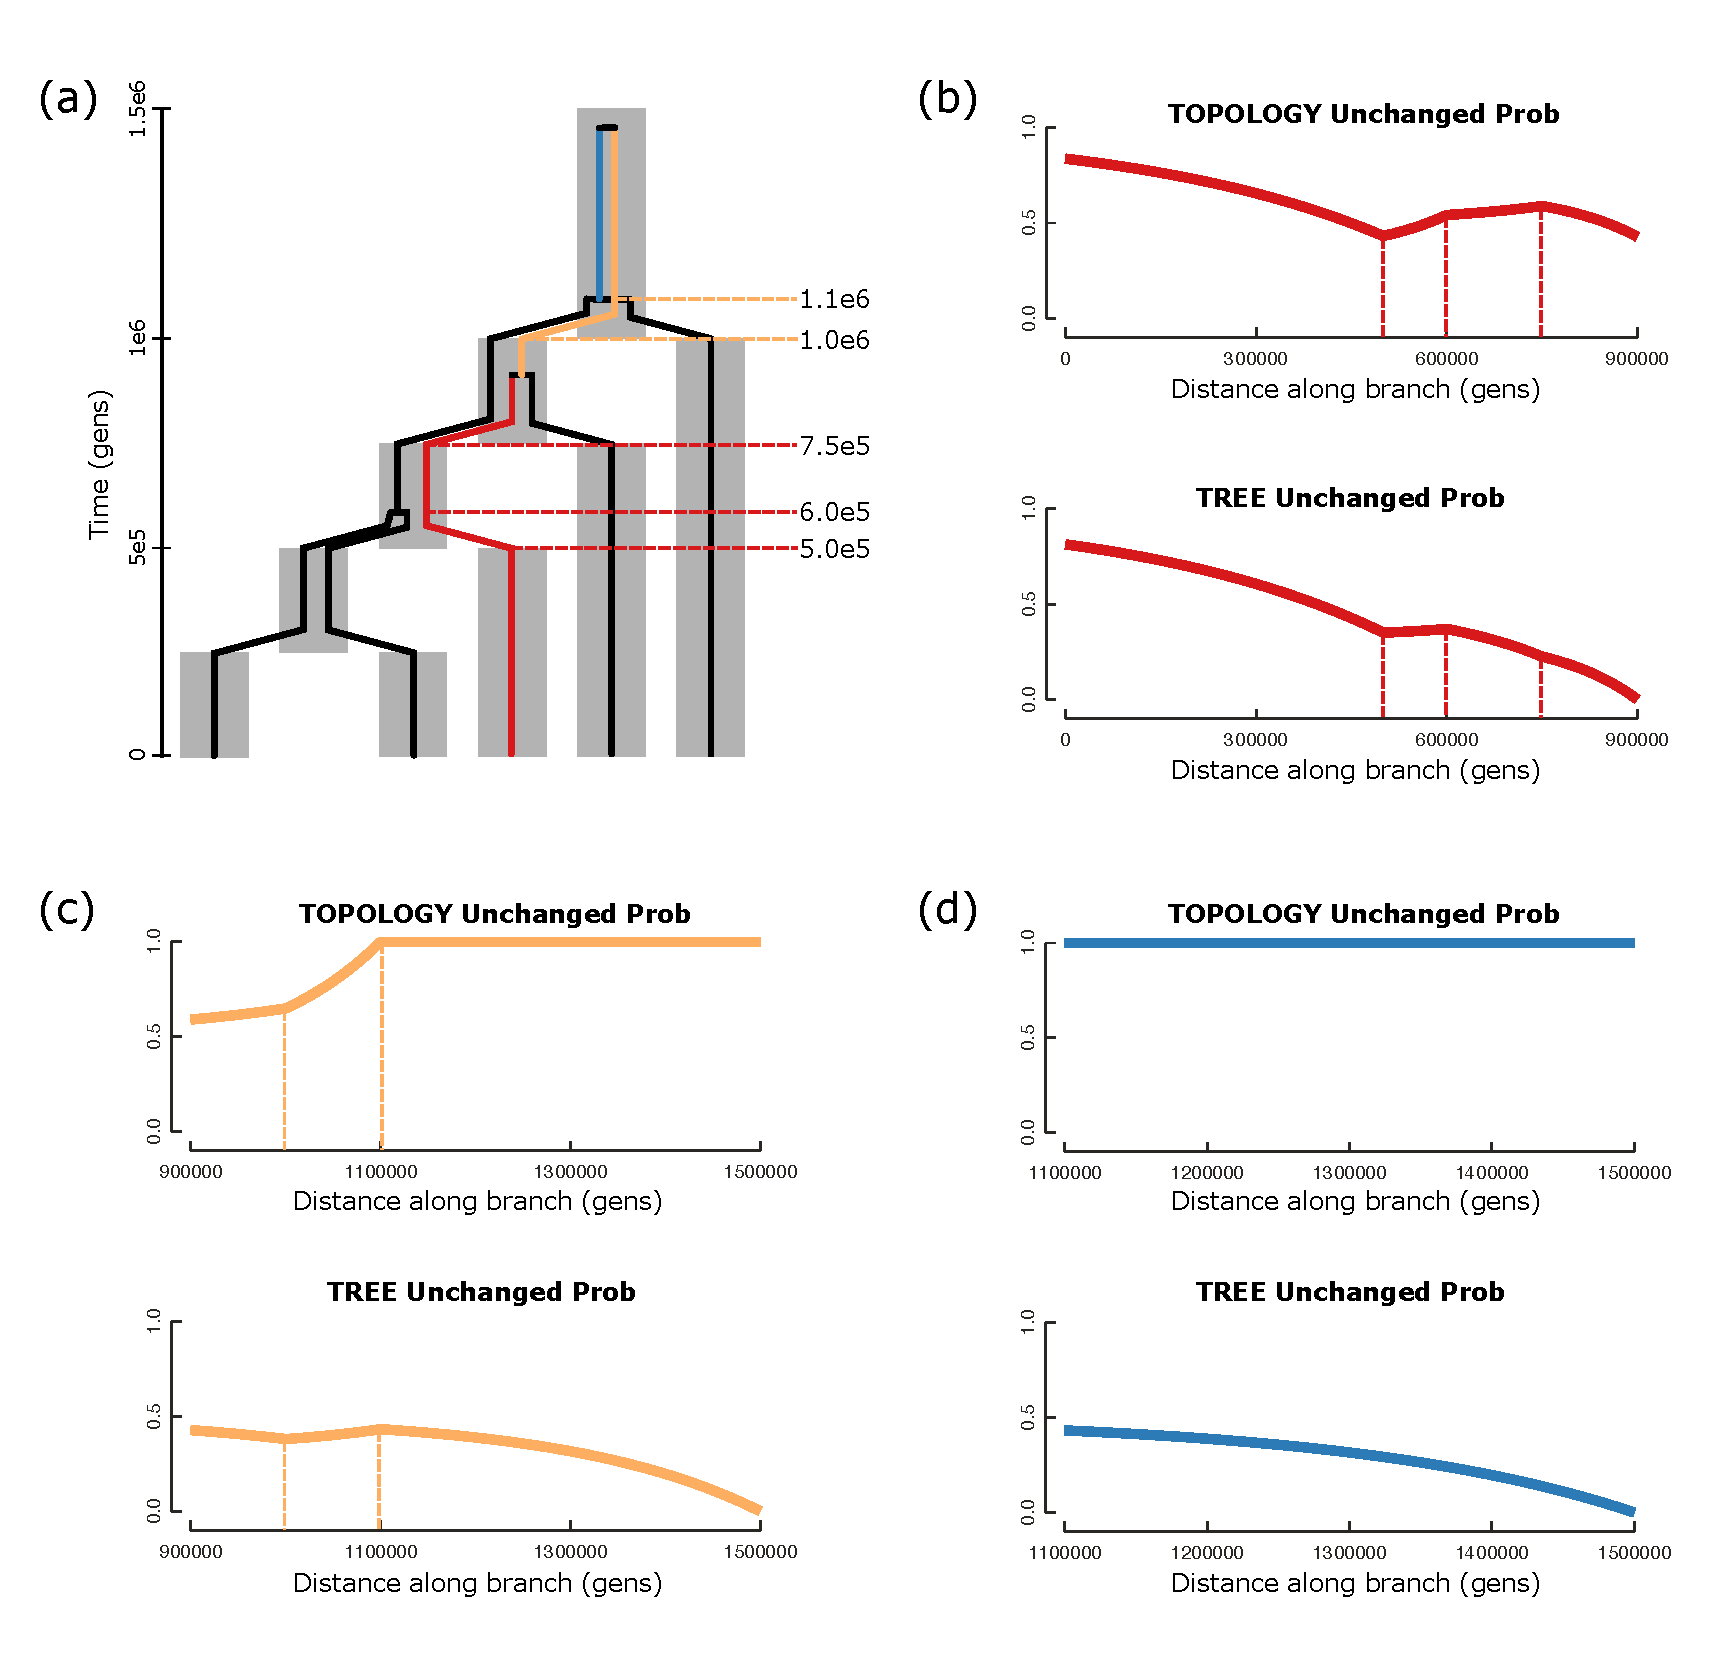
\includegraphics[width=0.9\textwidth]{figures/Fig4-bt_prob.pdf}
	\caption{Probability that the topology and the tree remain unchanged, given a recombination event at a specific time on a specific branch. The species tree (a) was arbitrarily parameterized as being unbalanced with 5 tips, having internode distances of 2.5e5, and having constant Ne of 2e5. The embedded genealogical tree was randomly generated by \emph{ipcoal} using MSC probabilities. We selected three branches, indicated by three different colors, across which we calculated the probability that the topology would remain unchanged and the tree would remain unchanged if a recombination event were to occur at each time point on the branch (b-d). Dashed lines indicate the beginning and ending times of different intervals on each branch -- that is, either a relevant species tree divergence event or genealogy coalescence event.}
	% \label{fig:fig2}
\end{figure}

Next, we tested the effect of variation in basic species tree parameters on expected waiting distances to tree changes and topology changes (\textbf{Figure 4}). We started with four different species trees: two imbalanced and two balanced. For each pair, there is a large tree (10 tips), and a small tree (5 tips) pruned from the large tree, with internode distances kept the same. On each species tree, we generated 1000 random MSC genealogies using each of 9 different Ne values, ranging from 50000 to 250000. We calculated the expected waiting distance to a tree change and to a topology change for each genealogy/species tree pair, assuming a recombination rate of 1e-9 recombs/bp/generation. In Figure 4, we show the mean expected waiting distances to tree and topology changes for each species tree and for each Ne value. The decline in expected waiting distances across Ne values and from small to large trees demonstrates that, on average, waiting distances to tree and topology changes decrease with increasing numbers of tips sampled and with increasing Ne values. 

\begin{figure}
	\centering
	%\fbox{\rule[-.5cm]{4cm}{4cm} \rule[-.5cm]{4cm}{0cm}}
	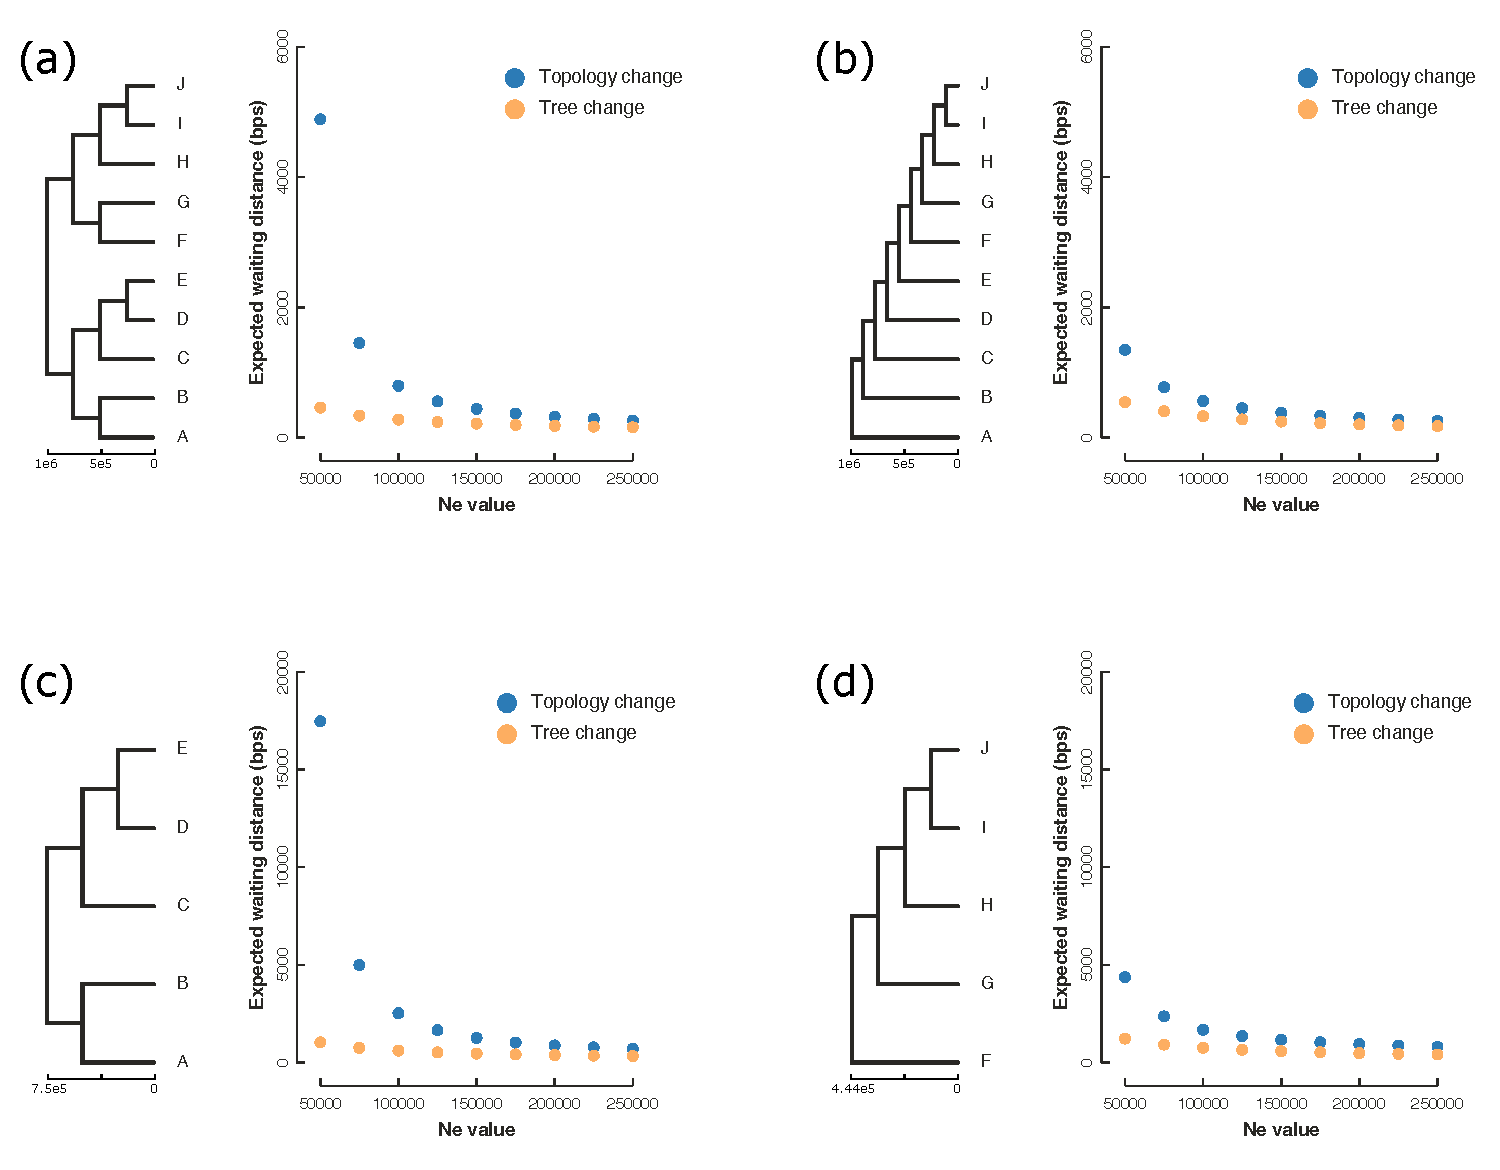
\includegraphics[width=0.9\textwidth]{figures/Fig5-waiting_times_ne_means.pdf}
	\caption{Mean expected waiting distances for differently parameterized species tree models. We used four different species trees: two 10-tip trees (a, b), each with 1e6-generation root heights, and two 5-tip trees (c, d) that are subselected from each of the larger trees. For each species tree, we iterated over 9 Ne values ranging from 50000 to 250000, generating 1000 unlinked MSC genealogies at each Ne value and calculating the expected waiting distance to a tree change and to a topology change for each. The mean of the expected waiting distances at each Ne value is presented in the scatterplot accompanying each species tree. Note that the y-axis scale changes from the top row (a, b) to the bottom row (c, d).}
	% \label{fig:fig3}
\end{figure}


Finally, we demonstrated that a known sequence of genealogies paired with the accompanying observed waiting distances to next topological change for each can be used to estimate the Ne value for species trees with different topologies (\textbf{Figure 5}). We used two different species trees: one imbalanced, 5-tip tree with internode branches of equal length, and one 10-tip tree with an irregular topology and branches of variable lengths. Both species trees were assigned equal root heights of 1e6 generations and equal Ne values of 150000 on all branches, and we simulated a 5e6-bp chromosome for each using \emph{ipcoal}. We broke each chromosome down into its component "initial genealogies" -- those that start each segment bounded by changes in topology -- and the accompanying segment lengths (i.e. waiting distances). Using these values and a known recombination rate of 1e-9 recombs/bp/generation, we calculated the likelihood that each of 41 proposed Ne values produced the set of genealogies and waiting distances. Using this approach, we recovered a correctly inferred Ne value of 150000 for both trees.

\begin{figure}
	\centering
	%\fbox{\rule[-.5cm]{4cm}{4cm} \rule[-.5cm]{4cm}{0cm}}
	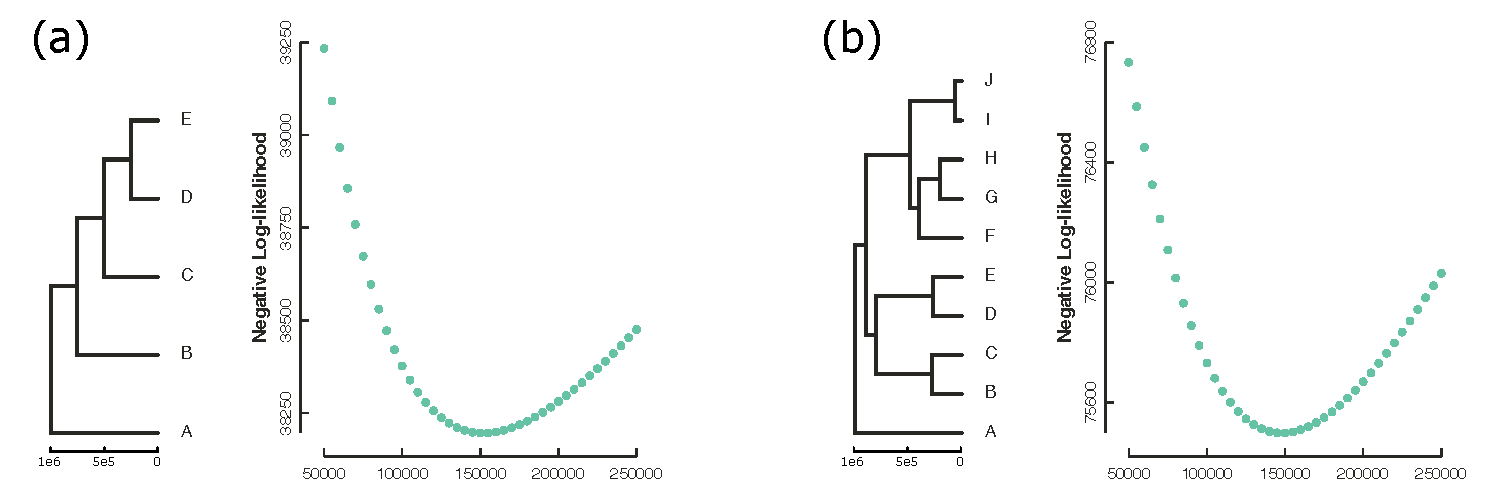
\includegraphics[width=0.9\textwidth]{figures/Fig6-constant_ne_inf.pdf}
	\caption{Inference of species tree Ne values from genealogies, observed waiting distances to topology changes, and recombination rate. We generated two different species trees: Both have root heights of 1e6 generations, but one has five tips, an unbalanced topology, and identical internode lengths, while the other has ten tips, an irregular topology, and irregular branch lengths. Using a recombination rate of 1e-9 recombs/bp/generation and a constant Ne value of 150000 over all branches, we generated a 5MB tree sequence from each species tree using \emph{ipcoal}. Then, we decomposed the alignment into segments bounded by topology changes in the genealogies, and we recorded the initial genealogy for each segment. Finally, we calculated the likelihood of the set of genealogies and waiting distances, along with the recombination rate, at 41 different proposed Ne values. For both sequence alignments, 150000 was correctly inferred as the Ne value.}
	% \label{fig:fig4}
\end{figure}

\section{Conclusions}
% \label{sec:others}

By accounting for the genomic heterogeneity that is expected due to incomplete lineage sorting, the multispecies coalescent model has facilitated the widespread use of multilocus data for phylogenetic inference. As phylogenetic systematics continues to turn toward whole genomes, methods should seek to take advantage of the increased resolution offered by genomic data. The traditional multispecies coalescent model overlooks the process of recombination, assuming that loci represent a single genetic history and that they are completely unlinked. In reality, under a neutral model, species tree parameters and recombination rates will influence the degree of genealogical turnover along a chromosome, potentially resulting in linked loci and/or multiple genealogical topologies per locus. Therefore, not accounting for recombination might mislead analyses. Conversely, incorporating the rates of turnover observed in the data as information could offer further clues for inference of the species tree model that generated it. 

 We began with a simple question: what is the expected turnover rate in topologies along a genome under a species tree model? We generalized a recent solution that used a single population and constant Ne, instead structuring the equations to accept an arbitrary species tree topology and a different, arbitrary Ne value for each species tree branch. These solutions lay a groundwork for exploring how species tree structures affect neutral expectations of genealogical heterogeneity across chromosomes.

%Inference of genealogies along a chromosome is a common goal in population genetics, and similar efforts have been undertaken in phylogenetics. Often, the goal of such efforts is to detect signals of introgression or selection. However, the phylogenetic approaches usually do not explicitly incorporate a model for recombination \citep[e.g.,][]{li2019recombination}. A notable exception to this is ARGweaver-D, which accepts models with population divergence and migration event parameters. Rather than derive probabilities of sequences of genealogical trees, ARGweaver-D uses an MCMC to sample the sequences. This approach is a powerful extension of the single-population ARGweaver method and has been applied successfully to study evolution of hominins, but it is limited to small numbers of samples. Challenges remain for studying properties of tree sequences for larger sets of samples.

Inference of genealogies along a chromosome is a common goal in population genetics, and similar efforts have been undertaken in phylogenetics. Often, the goal of such efforts is to detect signals of introgression or selection. However, the phylogenetic approaches usually do not explicitly incorporate a model for recombination \citep[e.g.,][]{li2019recombination}. Applications of our solutions might provide valuable null hypotheses of genealogical turnover rates by which introgression or selection might be detected. Beyond its use for detecting patterns resulting from non-neutral processes, incorporating recombination in phylogenetic-scale models could also help improve species tree inference. For example, to the extent that they are observable, the empirical distribution of waiting distances to topology changes might be inferred and compared against the expected waiting distances for a proposed species tree model (e.g., \textbf{Figure 5}). Further approaches could determine the distribution of waiting distances to specific types of topology changes, such as those that split up a focal clade.

%\subsection{Citations}
%Citations use \verb+natbib+. The documentation may be found at
%\begin{center}
%	\url{http://mirrors.ctan.org/macros/latex/contrib/natbib/natnotes.pdf}
%\end{center}

%Here is an example usage of the two main commands (\verb+citet+ and \verb+citep+): Some people thought a thing \citep{kour2014real, hadash2018estimate} but other people thought something else \citep{kour2014fast}. Many people have speculated that if we knew exactly why \citet{kour2014fast} thought this\dots

%\subsection{Figures}
%\lipsum[10]
%See Figure \ref{fig:fig1}. Here is how you add footnotes. %\footnote{Sample of the first footnote.}
%\lipsum[11]

%\begin{figure}
%	\centering
	%\fbox{\rule[-.5cm]{4cm}{4cm} \rule[-.5cm]{4cm}{0cm}}
%	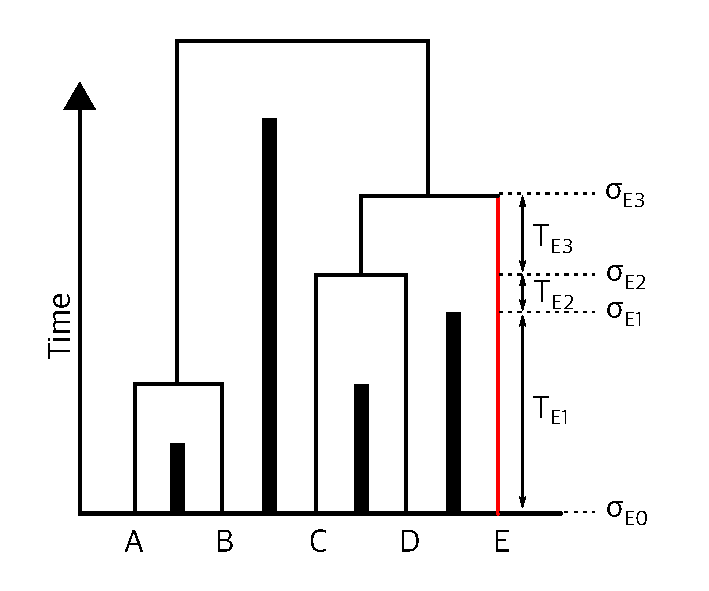
\includegraphics[width=0.6\textwidth]{genealogy_ebranch.pdf}
%	\caption{Sample figure caption.}
%	\label{fig:fig1}
%\end{figure}

%\subsection{Tables}
%See awesome Table~\ref{tab:table}.

%The documentation for \verb+booktabs+ (`Publication quality tables in LaTeX') is available from:
%\begin{center}
%	\url{https://www.ctan.org/pkg/booktabs}
%\end{center}


%\begin{table}
%	\caption{Sample table title}
%	\centering
%	\begin{tabular}{lll}
%		\toprule
%		\multicolumn{2}{c}{Part}                   \\
%		\cmidrule(r){1-2}
%		Name     & Description     & Size ($\mu$m) \\
%		\midrule
%		Dendrite & Input terminal  & $\sim$100     \\
%		Axon     & Output terminal & $\sim$10      \\
%		Soma     & Cell body       & up to $10^6$  \\
%		\bottomrule
%	\end{tabular}
%	\label{tab:table}
%\end{table}

%\subsection{Lists}
%\begin{itemize}
%	\item Lorem ipsum dolor sit amet
%	\item consectetur adipiscing elit.
%	\item Aliquam dignissim blandit est, in dictum tortor gravida eget. In ac rutrum magna.
%\end{itemize}


\bibliographystyle{ecol_let}
\bibliography{references}  %%% Uncomment this line and comment out the ``thebibliography'' section below to use the external .bib file (using bibtex) .


%%% Uncomment this section and comment out the \bibliography{references} line above to use inline references.
% \begin{thebibliography}{1}

% 	\bibitem{kour2014real}
% 	George Kour and Raid Saabne.
% 	\newblock Real-time segmentation of on-line handwritten arabic script.
% 	\newblock In {\em Frontiers in Handwriting Recognition (ICFHR), 2014 14th
% 			International Conference on}, pages 417--422. IEEE, 2014.

% 	\bibitem{kour2014fast}
% 	George Kour and Raid Saabne.
% 	\newblock Fast classification of handwritten on-line arabic characters.
% 	\newblock In {\em Soft Computing and Pattern Recognition (SoCPaR), 2014 6th
% 			International Conference of}, pages 312--318. IEEE, 2014.

% 	\bibitem{hadash2018estimate}
% 	Guy Hadash, Einat Kermany, Boaz Carmeli, Ofer Lavi, George Kour, and Alon
% 	Jacovi.
% 	\newblock Estimate and replace: A novel approach to integrating deep neural
% 	networks with existing applications.
% 	\newblock {\em arXiv preprint arXiv:1804.09028}, 2018.

%\end{thebibliography}

\section{Appendix: Step-by-Step Solution}


\subsection{Notation Summary}

\hl{make a table to summarize the notation here. Much easier to read than the itemized method currently.}

\subsection{Notation}

Assume we have sampled from a species tree $\mathcal{S}$ with $\mathcal{N}$ tips, where 
each tip represents a sampled individual belonging to one of the species. The species tree 
consists of a topology describing the history of population divergences, where each branch 
of the topology has a constant effective diploid population size $N_b$ associated with it. 
Within each branch, coalescence occurs at a constant per-generation rate of $\frac{1}{2N_b}$. 

We begin with a genealogical tree $\mathcal{G}$ sampled from the species tree according 
to coalescent probabilities. This tree is embedded within the species tree so that the 
time of coalescence for any two individuals from different species in $\mathcal{G}$ 
is constrained to occur farther back in time than their species' coalescence times 
in $\mathcal{S}$.

In \citet{deng_distribution_2021}, the genealogical tree was broken into a series of 
intervals so that the number of remaining (not-coalesced) lineages was constant within
each interval. In their method, the number of remaining lineages decreases monotonically
through time from tipward to rootward intervals as lineages coalesce. Our approach is 
similar, except that the intervals are branch-specific and correspond to intervals of 
constant numbers of lineages to coalesce with ($A$) and constant effective population 
size ($N$). Breakpoints may therefore exist where divergences occur in the species 
tree (potentially changing both $A$ and $N$) and where coalescent events occur in 
the genealogical tree (reducing $A$). Unlike in \citet{deng_distribution_2021}, $A$ 
is no longer monotonic, since \emph{species} coalescent events can increase the number
of lineages available for coalescence, while \emph{genealogical} coalescent events
always reduce that number. 

The intervals within each branch of $\mathcal{T}$ are each assigned an index increasing
from $0$ to $\mathcal{I}_b-1$, where $\mathcal{I}_b$ is the total number of intervals
in the branch. The times in generations marking the lower and upper bounds of each 
branch $b$ are notated $t_l^b$ and $t_u^b$, respectively. Each interval of index $x$
is bounded by times $\sigma_x$ and $\sigma_{x+1}$.

\subsection{The distribution of distances to any change in a genealogical tree}
Our goal is to derive a distribution of waiting distances to the next tree change
from an input species tree and current genealogical tree.

\subsubsection{Given a branch and a time}
We begin by assuming a specific branch and time of a recombination event. We then 
integrate across possible times on that branch, and we sum across all branches on
the tree to solve for the probability of the genealogy being unchanged given any 
recombination event. Finally, we incorporate this probability into the exponential
distribution presented in Equation 4.

\begin{equation}
	\mathbb{P}(\textrm{tree unchanged} | b,t,\mathcal{T},\mathcal{S}) = 
	\int_{t}^{t^u_b}\frac{1}{A(\tau)}p(\tau|t)d\tau
\end{equation}

Where $A(\tau)$ is the number of lineages able to be coalesced with at any time $\tau$, 
and $p(\tau|t_r)$ is the exponential probability density of coalescing any time 
after the recombination event. Thus, we are integrating over the probability
of coalescence along the path of species tree intervals traversed
by branch $b$, starting at the time of recombination and ending at the 
end of the branch. If the branch spans only a single gene tree embedding 
interval then $A(\tau)$ and $N(\tau)$

Through this series of one or more gene tree embedding intervals the 

up to that time through the species tree intervals that are traversed
by branch $b$, which can involve changing numbers of samples over time (A(t)), 
and changing effective population sizes (N(t)).
Here we define the coalescence rate at time $\tau$ as $\frac{A(\tau)}{N(\tau)}$. 
Note that this differs from \citet{deng_distribution_2021}, 
since our branch lengths are in units of generations rather than in
coalescent units. 

% who defined the 
% coalescent rate over an interval using the more common compound 
% metric of coalescent time units (time in generations /2N). 
% For the purposes of our equations it is simpler to  better to define define time in generations from the
% coalescent probability at any unit of time. per unit
% time, 


% coalescence rate.

\begin{equation}
	= \int_{t}^{t^u_b}\frac{1}{A(\tau)} \frac{A(\tau)}{N(\tau)}
	e^{-\int_t^\tau{}\frac{A(s)}{N(s)}ds} d\tau
\end{equation}


\begin{equation}
	= \int_{t}^{t^u_b}\frac{1}{N(\tau)}e^{-\int_t^\tau{}\frac{A(s)}{N(s)}ds} d\tau
\end{equation}



We can now take advantage of the fact that the rate of coalescence is piecewise-constant. We split the equation into one interval $i$ whose length depends on $t$ (it ranges from $t$ until the upper limit of its interval, $\sigma_{i+1}$) and we add to it integrals across intervals that are above it on the same branch, which are predefined by their upper and lower $\sigma$ values:

\begin{equation}
	= \int_{t}^{\sigma_{i+1}} \frac{1}{N(\tau)}\exp\left(-\int_{t}^{\tau}\frac{A(s)}{N(s)}ds\right)d\tau + \sum_{k=i+1}^{\mathcal{I}_b-1}\int_{\sigma_{k}}^{\sigma{k+1}}\frac{1}{N(\tau)}\exp\left(-\int_{t}^{\tau}\frac{A(s)}{N(s)}ds\right)d\tau
\end{equation}

We solve first term and later terms separately:

\paragraph{First term --}

\begin{equation}
	= \frac{1}{a_i} - \frac{1}{a_i}e^{-\frac{a_i}{n_i}\sigma_{i+1}}e^{\frac{a_i}{n_i}t}
\end{equation}

\begin{equation}
	= \frac{1}{a_i} +P_{ii}e^{\frac{a_i}{n_i}t}
\end{equation}

\paragraph{Later terms --}

\begin{equation}
	= \sum_{k=i+1}^{\mathcal{I}_b-1} e^{\frac{a_i}{n_i}t} \exp\left(-\frac{a_i}{n_i}\sigma_{i+1}-\sum_{q=i+1}^{k-1} \frac{a_q}{n_q}T_q\right)\left(\frac{1}{a_{k}}(1-e^{-\frac{a_{k}}{n_{k}}T_{k}})\right)
\end{equation}

\begin{equation}
	= \sum_{k=i+1}^{\mathcal{I}_b-1} e^{\frac{a_i}{n_i}t} P_{ik}
\end{equation}

Where:
\begin{itemize}
  \item $i$ is the interval index to which $t$ belongs
  \item $a_x$ is the value of A(t) for all $t$ in interval $x$
  \item $n_x$ is the value of N(t) for all $t$ in interval $x$
  \item $T_x = \sigma_{x+1} - \sigma_{x}$
  \item $\mathcal{I}_b$ is the number of intervals on branch $b$
  \item $\mathcal{T}$ is the current genealogy, and 
  \item $\mathcal{S}$ is the species tree with divergence times and branch-specific effective population sizes.
\end{itemize}

Adding these together, we are left with the solution:

\begin{equation}
	\mathbb{P}(\textrm{tree unchanged} | b,t,\mathcal{T},\mathcal{S}) = \frac{1}{a_i}+\sum_{k=i}^{\mathcal{I}_b-1}{P_{ik}e^{\frac{a_i}{n_i}t}}
\end{equation}

\subsubsection{Across a full branch}

Having solved for the probability of the genealogical tree being unchanged given the time $t$ of the recombination event, our next step is to integrate this equation across the branch with respect to $t$:

\begin{equation}
	\mathbb{P}(\textrm{tree unchanged} | b,\mathcal{T},\mathcal{S}) = \frac{1}{t^u_b-t^l_b} \int_{t_b^l}^{t_b^u} \mathbb{P}(\textrm{tree unchanged} | b,t,\mathcal{T},\mathcal{S})dt
\end{equation}

Plugging in Equation 17 above, we find:

\begin{equation}
	= \frac{1}{t^u_b-t^l_b}\sum_{i=0}^{\mathcal{I}_b-1}\frac{1}{a_i}T_i + \left(e^{\frac{a_i}{n_i}\sigma_{i+1}}-e^{\frac{a_i}{n_i}\sigma_i}\right)\left[-\frac{n_i}{a_i^2}e^{-\frac{a_i}{n_i}\sigma_{i+1}} + \frac{n_i}{a_i}\left(\sum_{k=i+1}^{\mathcal{I}_b-1}\exp\left(-\frac{a_i}{n_i}\sigma_{i+1}-\sum_{q = i+1}^{k-1}\frac{a_q}{n_q}T_q\right)\frac{1-\exp(-\frac{a_{k}}{n_{k}}T_{k})}{a_{k}}\right)\right]
\end{equation}

\subsubsection{Across the whole tree}

At last, we can calculate the probability that, given a recombination event, the genealogical tree is unchanged. We do this by weighting each branch by its proportion of the total tree length and summing across the unchanging probabilities for all branches:

\begin{equation}
	\mathbb{P}(\textrm{tree unchanged} | \mathcal{T},\mathcal{S}) = \sum_{b=1}^{2N-2}\left[\frac{t^u_b-t^l_b}{L(\mathcal{T})}\right]\mathbb{P}(\textrm{tree unchanged} | b,\mathcal{T},\mathcal{S})
\end{equation}

To derive the waiting distance to the next tree change, we incorporate the value of $1-\mathbb{P}(\textrm{tree unchanged} | \mathcal{T},\mathcal{S})$ into the exponential distribution describing the waiting distance to the next recombination event (introduced in Equation 4):
\begin{equation}
\begin{aligned}
	&p_r(d|\mathcal{T},\mathcal{S}) = r\alpha_\mathcal{S}(\mathcal{T})L(\mathcal{T})\exp\left[-r\alpha_\mathcal{S}(\mathcal{T})L(\mathcal{T})d\right]\textrm{,} \\
	&where \\
	&\alpha_\mathcal{S}(\mathcal{T})=1-\mathbb{P}(\textrm{tree unchanged} | \mathcal{T},\mathcal{S}).
\end{aligned}
\end{equation}

\subsection{The distribution of distances to a change in genealogical topology}

Next, we attempt to further exclude recombination events. We filter out recombination events of categories 2 and 3, which just change branch lengths, to isolate the probability that a recombination event changes the \emph{topology} of the tree.

As in the first section, we treat branches individually and then sum across them. However, we have to designate new variables. We now consider two lineages in addition to the focal lineage $b$: the lineage $b'$ that $b$ coalesces with, and the lineage $c$ that is ancestral to $b$ and $b'$. We also designate the timepoint $t_b^m$, which we use to break the problem into two cases. While the single-population example in \citet{deng_distribution_2021} uses $t_{b'}^l$ as this breakpoint, the species tree introduces more complexity, and we instead use the maximum of three values: $t_{b'}^l$, $t_{b}^l$, and $t_{(b,b')}^w$, which we define as the merging time for the species tree branches separating $b$ and $b'$ (Figure 6).

\begin{figure}
	\centering
	%\fbox{\rule[-.5cm]{4cm}{4cm} \rule[-.5cm]{4cm}{0cm}}
	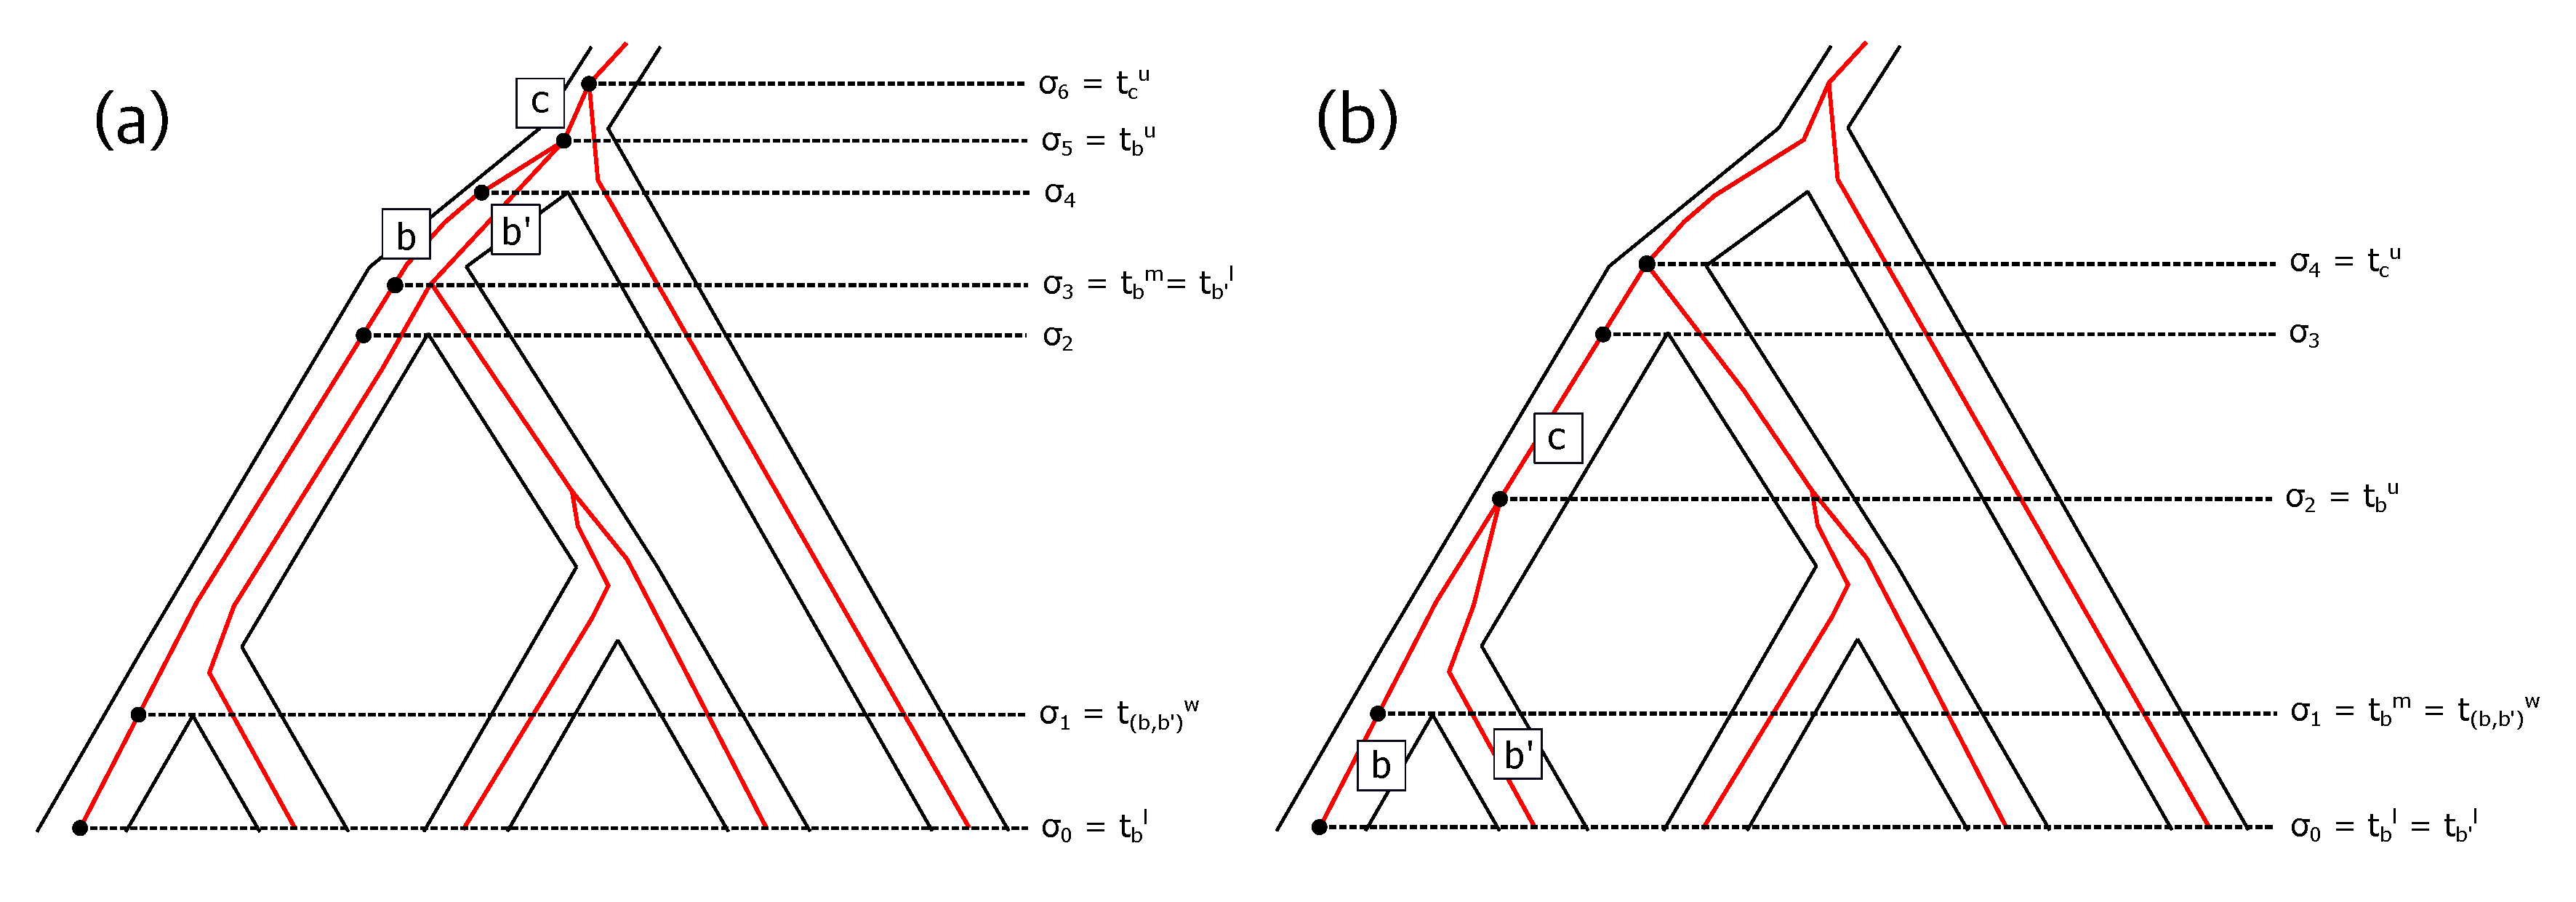
\includegraphics[width=0.9\textwidth]{figures/FigS1-topology_illustration.pdf}
	\caption{Illustrating the parameters for calculating the distribution of distances to a change in the topology of a genealogy. Panels (a) and (b) show slightly different genealogies embedded in the same species tree. In both (a) and (b), the focal branch $b$ is the one leading from the left-most species. Branches $c$ and $b'$ -- the parent and sibling branches, respectively -- are also both labeled. Note that in (a), $t_b^m$ corresponds to $\sigma_3$, while in (b) it corresponds to $\sigma_1$.}
	% \label{fig:fig5}
\end{figure}

\begin{equation}
	\mathbb{P}(\textrm{topology unchanged} | b,\mathcal{T},\mathcal{S}) = \frac{1}{t_b^u-t_b^l}\int_{t_b^l}^{t_b^u}\mathbb{P}(\textrm{topology unchanged} | b,t,\mathcal{T},\mathcal{S})dt
\end{equation}

\begin{equation}
	= \frac{1}{t_b^u-t_b^l}\left[\left(\int_{t_b^l}^{t_b^m}+\int_{t_b^m}^{t_b^u}\right)\mathbb{P}(\textrm{topology unchanged} | b,t,\mathcal{T},\mathcal{S})dt\right]
\end{equation}

Where $t^m_b=\max\{t^w_{(b,b')},t_{b'}^l,t_b^l\}$.

\subsubsection{Given a branch and a time}

As in \citet{deng_distribution_2021}, we break the problem into two cases: a first case in which $t$ belongs to the interval from the base of the focal branch to $t^m_b$, and a second case in which $t$ belongs to the interval from $t^m_b$ to $t^u_b$. 

\paragraph{First case --} Given $t \in [\sigma_i, \sigma_{i+1}] \subset [t_b^l,t_{b}^m]$:

\begin{equation*}
	\mathbb{P}(\textrm{topology unchanged} | b,t,\mathcal{T},\mathcal{S}) = \int_{t}^{t_b^m}\frac{1}{A(\tau)}\rho(\tau|t)d\tau + \int_{t_b^m}^{t_b^u}\frac{2}{A(\tau)}\rho(\tau|t)d\tau + \int_{t_b^u}^{t_c^u}\frac{1}{A(\tau)}\rho(\tau|t)d\tau
\end{equation*}

\begin{equation}
	= \frac{1}{a_i} + \sum_{k=i}^{\mathcal{I}_{b+c}-1}P_{ik}e^{\frac{a_i}{n_i}t} + \sum_{k=m}^{\mathcal{I}_b-1}P_{ik}e^{\frac{a_i}{n_i}t}
\end{equation}

The second case is solved in a similar manner, although we eliminate the first integral:

\paragraph{Second case --} Given $t \in [\sigma_i, \sigma_{i+1}] \subset [t_b^m,t_b^u]$:

\begin{equation*}
	\mathbb{P}(\textrm{topology unchanged} | b,t,\mathcal{T},\mathcal{S}) = \int_{t}^{t_b^u}\frac{2}{A(\tau)}\rho(\tau|t)d\tau + \int_{t_b^u}^{t_c^u}\frac{1}{A(\tau)}\rho(\tau|t)d\tau
\end{equation*}

\begin{equation}
	= 2\left(\frac{1}{a_i} + \sum_{k=i}^{\mathcal{I}_{b}-1}P_{ik}e^{\frac{a_i}{n_i}t}\right) + \sum_{\mathcal{I}=n_b}^{\mathcal{I}_{b+c}-1}P_{ik}e^{\frac{a_i}{n_i}t}
\end{equation}

\subsubsection{Across a full branch}

Now we derive the overall probability that a recombination event falling on a specific branch will change the topology. We integrate across values of $t$ and sum the two cases defined above, while assuming a uniform probability of the recombination event occurring at any time along the branch:

\paragraph{First case --}

\begin{equation}
	\int_{t_b^l}^{t_b^m}{\mathbb{P}(\textrm{topology unchanged} | b,t,\mathcal{T},\mathcal{S})}=\sum_{i=0}^{m-1}\frac{1}{a_i}\left[T_i+n_i\left(\exp\left(\frac{a_i}{n_i}\sigma_{i+1}\right)-\exp\left(\frac{a_i}{n_i}\sigma_i\right)\right)\left(\sum_{k=i}^{\mathcal{I}_{b+c}-1}P_{ik}+\sum_{k=m}^{\mathcal{I}_b-1}P_{ik}\right)\right]
\end{equation}

\paragraph{Second case --}

\begin{equation}
	\int_{t_b^m}^{t_b^u}{\mathbb{P}(\textrm{topology unchanged} | b,t,\mathcal{T},\mathcal{S})}=\sum_{i=m}^{\mathcal{I}_b-1}\frac{1}{a_i}\left[2T_i + n_i\left(\exp\left(\frac{a_i}{n_i}\sigma_{i+1}\right)-\exp\left(\frac{a_i}{n_i}\sigma_i\right)\right)\left(2\sum_{k=i}^{\mathcal{I}_b-1}P_{ik}+\sum_{k=\mathcal{I}_b}^{\mathcal{I}_{b+c}-1}P_{ik}\right)\right]
\end{equation}

\paragraph{Result --}
\begin{equation}
    \mathbb{P}(\textrm{topology unchanged}|b, \mathcal{T},\mathcal{S}) = \frac{1}{t_b^u-t_b^l}\left[\sum_{i=0}^{m-1}p_{b,1}^{(i)}+\sum_{i=m}^{\mathcal{I}_b-1}p_{b,2}^{(i)}\right]
\end{equation}

\subsubsection{Across the whole tree}

Finally, we sum across all branches to find the probability of a recombination event changing the topology of the tree:

\begin{equation*}
    \mathbb{P}(\textrm{topology unchanged}| \mathcal{T},\mathcal{S}) = \sum_{b=1}^{2N-2}\frac{t_b^u-t_b^l}{L(\mathcal{T})} \times \mathbb{P}(\textrm{topology unchanged}|b, \mathcal{T},\mathcal{S})
\end{equation*}

\begin{equation}
    = \frac{1}{L(\mathcal{T})}\sum_{b=1}^{2N-2}\left[\sum_{i=0}^{m-1}p_{b,1}^{(i)}+\sum_{i=m}^{\mathcal{I}_b-1}p_{b,2}^{(i)}\right]
\end{equation}

\end{document}
